%------------------------------------------------------------------------------
% Template file for the submission of papers to IUCr journals in LaTeX2e
% using the iucr document class
% Copyright 1999-2013 International Union of Crystallography
% Version 1.6 (28 March 2013)
%------------------------------------------------------------------------------
%
%
\documentclass{iucr}
% \documentclass[preprint]{iucr}              % DO NOT DELETE THIS LINE
\usepackage{bm}
% \usepackage{graphicx}
% \usepackage{tabularx}
% \usepackage{subfigure}
% \usepackage{afterpage}
% \usepackage{sansmath}
\usepackage{mathtools}
\usepackage{array}
% \usepackage{parskip}
% \usepackage{tikz}
% \usepackage{tikzorbital}
% \usepackage{setspace}
% \usepackage{xcolor}
\usepackage{amssymb}
% \usepackage{bm}
\usepackage{amsmath}
% \usepackage{fancyhdr}
% \usepackage{rotating}
\usepackage{siunitx}
\usepackage{url}
\usepackage{color}
%\usepackage{cprotect}
\usepackage{textgreek}
\usepackage[normalem]{ulem}
\usepackage{makecell}
\usepackage{cancel}
\usepackage{empheq}
\usepackage[usenames,dvipsnames]{xcolor}


% %%%%%%%%%%%%%%%%
% \usepackage[utf8]{inputenc}
% \usepackage[]{graphicx}
% \usepackage{rotating}
% \usepackage{hyperref}
% \usepackage{listings}

% \lstset{language=Fortran,
%         keywordstyle=\color{blue}\textbf,
% 	commentstyle=\color[rgb]{0.133,0.545,0.133},
% 	stringstyle=\color[rgb]{0.627,0.126,0.941},
% 	breaklines=true,
% 	showstringspaces=false,
% 	frame=trBL, basicstyle=\scriptsize %\small %\tiny %\footnotesize
%        }
% %%%%%%%%%%%%%%%%


\definecolor{darkblue}{rgb}{0.0, 0.0, 0.55}
\definecolor{cyan(process)}{rgb}{0.0, 0.72, 0.92}

\newcommand{\todo}[1]{{\color{red}[TODO: "#1'']}}
\newcommand{\inblue}[1]{{\color{blue}#1}}
\newcommand{\cyan}[1]{{\color{cyan(process)}#1}}
\newcommand{\inred}[1]{{\color{red}#1}}
\newcommand{\ingreen}[1]{{\color{green}#1}}


%%%%%%%%%%%%%%%%%%% subsubsubsection (see: https://tex.stackexchange.com/questions/60209/how-to-add-an-extra-level-of-sections-with-headings-below-subsubsection )
% \setcounter{secnumdepth}{5}
% \setcounter{tocdepth}{5}

% \makeatletter
% \newcommand\subsubsubsection{\@startsection{paragraph}{4}{\z@}{-2.5ex\@plus -1ex \@minus -.25ex}{1.25ex \@plus .25ex}{\normalfont\normalsize\bfseries}}
% \newcommand\subsubsubsubsection{\@startsection{subparagraph}{5}{\z@}{-2.5ex\@plus -1ex \@minus -.25ex}{1.25ex \@plus .25ex}{\normalfont\normalsize\bfseries}}
% \makeatother
%%%%%%%%%%%%%%%%%%%
\makeatletter
\@ifclasswith{iucr}{preprint}{
\newcommand{\whencolumns}[2]{#1}
}{
\newcommand{\whencolumns}[2]{#2}
}
\makeatother

     %-------------------------------------------------------------------------
     % Infobrmation about journal to which submitted
     %-------------------------------------------------------------------------
     \journalcode{X}              % Indicate the journal to which submitted
                                  %   A - Acta Crystallographica Section A
                                  %   B - Acta Crystallographica Section B
                                  %   C - Acta Crystallographica Section C
                                  %   D - Acta Crystallographica Section D
                                  %   E - Acta Crystallographica Section E
                                  %   F - Acta Crystallographica Section F
                                  %   J - Journal of Applied Crystallography
                                  %   M - IUCrJ
                                  %   S - Journal of Synchrotron Radiation

\begin{document}  % DO NOT DELETE THIS LINE

\title{Ray tracing of polarized light in SHADOW4: application to polarizers and phase shifters for X-rays and visible light}

\cauthor[1]{{Manuel}}{{Sanchez del Rio}}{srio@esrf.eu}{address if different from \aff}
\author[1]{{Carsten}}{{Detlefs}}
\author[1]{{Daniel}}{{Fiole}}
\author[2]{{Sonia}}{{Francoual}}
\author[3]{{Luca}}{{Rebuffi}}
\author[4]{{Juan}}{{Reyes-Herrera}}
\author[5]{{Xiaojiang}}{{Yu}}


\aff[1]{ESRF - The European Synchrotron, 71 Avenue des Martyrs, 38000 Grenoble, \country{France}}
\aff[2]{Deutsches Elektronen-Synchrotron DESY, Notkestra{\ss}e 85, 22607 Hamburg, \country{Germany}}
\aff[3]{Argonne National Laboratory, 9700 S. Cass Avenue, Lemont, IL 60439, \country{USA}}
\aff[4]{Elettra -- Sincrotrone Trieste, S.S. 14 km 163.5 in AREA Science Park, 34149 Basovizza, Trieste, \country{Italy}}
\aff[5]{Singapore Synchrotron Light Source, National University of Singapore, 5 Research Link, Singapore 117603 \country{Singapore}}

\maketitle   % DO NOT DELETE THIS LINE

% -----------------------------------------------------------------
% -----------------------------------------------------------------

\begin{synopsis}
SHADOW4 tracks the complex $\sigma$ and $\pi$ amplitudes of the electric field of each ray and transforms them with Jones matrices. Examples cover polarizers and phase shifters for X-rays (perfect crystals, a new crystal phase plate) and for visible light (Brewster mirrors, Fresnel rhomb).
\end{synopsis}

% -----------------------------------------------------------------
% -----------------------------------------------------------------

\begin{abstract}
SHADOW4 stores in each ray the complex $\sigma$ and $\pi$ amplitudes of the electric field, and transforms them at every optical element with Jones matrices. We describe this formulation, from the polarization at the source to the change of reference frame between optical elements of any orientation. A new optical element computes the beam transmitted by a perfect crystal plate, making possible the simulation of X-ray phase plates. We illustrate the method with polarizers and phase shifters, using perfect crystals for X-rays and reflecting surfaces for visible light, and validate it against analytical and independent calculations.
\end{abstract}


% -----------------------------------------------------------------
% -----------------------------------------------------------------
\section{Introduction}\label{sec:introduction}
% -----------------------------------------------------------------
% -----------------------------------------------------------------

Ray tracing, combined with the Monte Carlo sampling of the source, has become an essential tool for designing, optimizing, and analyzing optical systems such as synchrotron radiation beamlines.
Many Monte Carlo codes store in each particle or ray an intensity or weight parameter, which is updated at every event.
Most electromagnetic interactions are described by the change of the electric field, therefore it is more appropriate to track the electric field rather than the intensity, which is the squared modulus of the field amplitudes.
The electric field permits to compute not only the intensity of each ray, but also its polarization and the phase changes. To extract usable and accurate information on these parameters, the electric field must be correctly simulated and propagated.
Here we look at the optical devices that change the polarization state of the beam, and we describe the models used to simulate them in the SHADOW4 \cite{ShadowSRN2023, SHADOW4} ray tracing package.
Other ray tracing codes for synchrotron beamlines also transport the polarization, e.g. RAY \cite{Schafers2008}, which uses Stokes vectors, and xrt \cite{Klementiev2014}, which uses complex field amplitudes.

SHADOW, already in its first version SHADOW1 \cite{Cerrina1984}, incorporated a full description of the electric field and phases: the two components of the electric field ($\sigma$, perpendicular to the scattering or diffraction plane, and $\pi$, parallel to it) are defined for each ray. This provided the infrastructure for a polarization-dependent treatment of the reflections in the optical elements (e.g. mirrors and perfect crystals). SHADOW2 \cite{Lai1988} included a model for plane crystals in Bragg (reflection) geometry, later upgraded to asymmetric crystals \cite{SanchezdelRio1992} and crystals in Laue (transmission) geometry \cite{SanchezdelRio1994}. In SHADOW3 \cite{codeSHADOW} and its ShadowOui interface \cite{codeSHADOWOUI}, the definition of the crystal parameters was made more user friendly, and external diffraction profiles can be used. SHADOW is therefore used to simulate a great variety of crystal optics: flat and curved crystals in Bragg and Laue geometries (monochromators, polychromators, analyzers), crystal polarizers at Bragg angles close to $45^\circ$, and many crystal structures, including those of interest for tender X-rays \cite{Yu_2022}.

The reflectivity of curved crystals is calculated in SHADOW3 (and still in SHADOW4) for the undistorted crystal, and some effects predicted by the dynamical theory (e.g., the focusing in the Borrmann triangle) are not included. Moreover, SHADOW3 only uses the diffracted beam of the crystals, while the dynamical theory predicts both a diffracted and a transmitted beam. This prevents the simulation of crystal phase shifters, which use the transmitted beam of a crystal plate set close to the Bragg angle.

With SHADOW4, a complete refactoring of this code, we have revisited and reimplemented the transport of the electric field. Each optical element is described by a Jones matrix applied in its own $\sigma$--$\pi$ frame, with an explicit change of frame between elements of any orientation. A new optical element computes the transmitted beam of a perfect crystal, which allows the simulation of X-ray phase plates. The formalism is not limited to crystals: polarization in mirrors and in the visible range (e.g. Brewster polarizers, Fresnel rhomb) is treated in the same way.

Section~\ref{sec:definitions} describes how the electric field is stored in the SHADOW rays, the conventions used, and how the Stokes parameters and the polarization ellipse are obtained. Section~\ref{sec:source} describes the polarization at the source. Section~\ref{sec:interaction} explains the changes of reference frame and the interaction with the optical elements using the Jones calculus. The following sections show examples of polarizers (section~\ref{sec:polarizers_all}) and phase shifters (section~\ref{sec:phaseshifters_all}), in the visible and X-ray ranges, including the new crystal phase plate of SHADOW4. The reflectivities of mirrors and crystals are summarized in Appendix~\ref{sec:mirrorandcrystals}, the method used in SHADOW3 in Appendix~\ref{sec:S3}, and the scripts used for the examples are listed in Appendix~\ref{sec:scripts}.


% -----------------------------------------------------------------
% -----------------------------------------------------------------
\section{Electric field of the rays and polarization conventions}\label{sec:definitions}
\subsection{SHADOW arrays and electric vectors}
% -----------------------------------------------------------------
% -----------------------------------------------------------------

A single ray $\vec{R}$ in SHADOW is an array of 18 parameters (called ``columns'' in SHADOW's jargon) stored in the following order:
\begin{equation}
   \vec{R}=( \vec{r},\vec{v},\vec{E}_\sigma,f,k,n,opd,\phi_\sigma,\phi_\pi,\vec{E}_\pi)^T,
\end{equation}
where $T$ is the transpose operator (we use ``column'' vectors), $\vec{r}=(x,y,z)^T$ are the spatial coordinates, $\vec{v}=(v_x,v_y,v_z)^T$ are the direction cosines (ray direction) with $|\vec{v}|=1$, $f$ is a flag (good or lost ray), $k$ is the wavevector modulus in $\mathrm{cm}^{-1}$ ($k=2\pi / \lambda$, with $\lambda$ the photon wavelength), $n$ is a counter (from one to the total number of rays), and $opd$ is the optical path (the travelled distance times the refractive index). The axes of the reference frame are $\hat{x}$, $\hat{y}$ and $\hat{z}$. The beam propagates along the $\hat{y}$ axis; $\hat{z}$ is usually vertical and $\hat{x}$ horizontal, completing a right-handed frame (Fig.~\ref{fig:S4_reference_frame}). Each beamline element has its own reference frame (section~\ref{sec:change_frame}).

\begin{figure}
    \centering
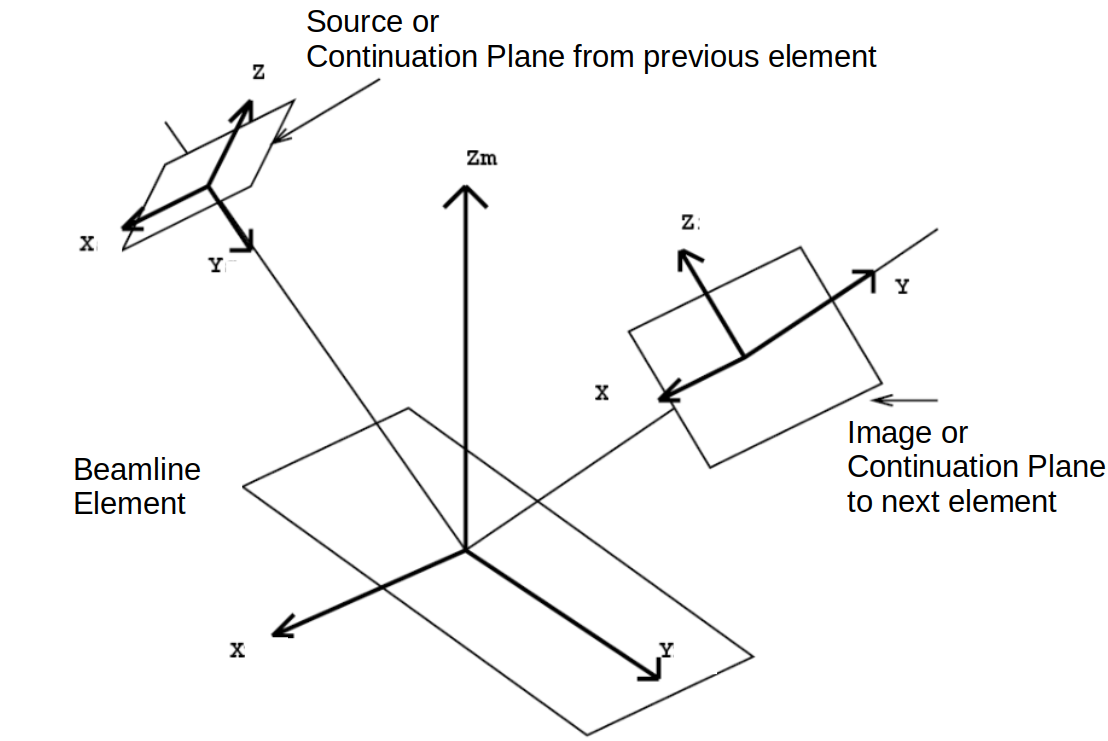
\includegraphics[width=0.9\linewidth]{figures/S4_reference_frame.png}
\caption{SHADOW4 reference frames: source, beamline element, and image coordinates. The rays are expressed in the frame of the source plane or of the image plane (continuation planes), with axes $X$, $Y$, $Z$ corresponding to $\hat{x}$, $\hat{y}$, $\hat{z}$ in the text: the beam propagates along $Y$. The frame of the beamline element ($Z_m$ is the normal to the surface) is described in section~\ref{sec:change_frame}. \todo{regenerate the figure with appropriated symbols}}
\label{fig:S4_reference_frame}
\end{figure}

The complex electric vector is expressed as a function of the $\sigma$ and $\pi$ components (perpendicular and parallel to the diffraction or reflection plane, respectively):

\begin{equation}\label{eq:electricfieldray}
   \vec{E}= \vec{E}_\sigma e^{i \phi_\sigma} + \vec{E}_\pi e^{i \phi_\pi},
\end{equation}
where the physical field is the real part of $\vec{E}e^{-i\omega t}$ (section~\ref{sec:polarization_stokes}). This equation can be expressed using the direction versors $\hat{u}_\sigma$ and $\hat{u}_\pi$\footnote{
They are calculated as
$\hat{u}_\sigma = \vec{E}_\sigma/|\vec{E}_\sigma|$ and $\hat{u}_\pi = (\hat{u}_\sigma \times \vec{v})/|\hat{u}_\sigma \times \vec{v}|$.
In case that $|\vec{E}_\sigma|=0$ the calculation is $\hat{u}_\pi = \vec{E}_\pi/|\vec{E}_\pi|$ and $\hat{u}_\sigma = (\vec{v} \times \hat{u}_\pi)/|\vec{v} \times \hat{u}_\pi|$. If $|\vec{E}|=0$ then we choose arbitrarily $\hat{u}_\sigma=\vec{v}\times\hat{z}$ (i.e., $\hat{u}_\sigma=\hat{x}$ for a ray along $\hat{y}$). This is computed in {\tt S4Beam.get\_efield\_directions}.
}
\begin{equation}\label{eq:electricfieldray2}
   \vec{E}=
    \mathcal{E}_\sigma \hat{u}_\sigma + 
    \mathcal{E}_\pi \hat{u}_\pi
   =
   E_\sigma e^{i \phi_\sigma} \hat{u}_\sigma + E_\pi e^{i \phi_\pi} \hat{u}_\pi
\end{equation}
with $\mathcal{E}_{\sigma,\pi}$ the complex amplitudes of the electric field and $E_{\sigma,\pi}=|\vec{E}_{\sigma,\pi}|$ the modulus of the complex amplitudes (real).

Note that the names $\sigma$ and $\pi$ are a convention (a definition) when applied to a ray: a ray travelling alone, at the source or between beamline elements, has no real diffraction or reflection plane. They only label two orthogonal directions perpendicular to $\vec{v}$. SHADOW chooses them as if the ray were going to be deflected in an ``imaginary'' diffraction plane, the vertical plane $(y,z)$, which is the deflection plane of a beamline element with orientation angle $\alpha=0$ (see section~\ref{sec:change_frame}). By default $\hat{u}_\sigma$ is along $\hat{x}$ (typically horizontal), perpendicular to the $(y,z)$ plane; and $\hat{u}_\pi$ lies in the $(y,z)$ plane. This holds exactly for a ray along $\hat{y}$, and approximately for divergent rays (see section~\ref{sec:source}). This flexibility in the directions of $\vec{E}_\sigma$ and $\vec{E}_\pi$ makes it possible to control the ray polarization in SHADOW precisely, and to propagate it along the optical components.
When the ray interacts with a beamline element, the real scattering plane, spanned by the incident and scattered directions, generally differs from this imaginary plane (for example, for a beamline element with $\alpha\neq 0$, or for divergent rays), and the electric field must be re-expressed in the $\sigma$ and $\pi$ directions of the real scattering plane, as described in section~\ref{sec:S4}.
% and of the electric fields for the $\sigma$ and  $\hat{u}_\pi$ can be calculated\footnote{this is done in {\tt S4Beam.get\_efield\_directions}.
% In case that $|\vec{E}_\sigma|=0$ the calculation is $\hat{u}_\pi = \vec{E}_\pi/|\vec{E}_\pi|$ and $\hat{u}_\sigma = (\vec{v} \times \hat{u}_\pi)/|\vec{v} \times \hat{u}_\pi|$. If $|\vec{E}|=0$ then we chose arbitrarly $\hat{u}_\sigma=(1,0,0)^T$.
% } as:
% \begin{eqnarray}
%     \hat{u}_\sigma = \frac{\vec{E}_\sigma}{|\vec{E}_\sigma|} \nonumber \\
%     \hat{u}_\pi = \frac{\hat{u}_\sigma \times \vec{v}}{|\hat{u}_\sigma \times \vec{v}|},
% \end{eqnarray}
% and equation~(\ref{eq:electricfieldray}) becomes 

The intensity carried by a single ray is (since $\vec{E}_\sigma \perp \vec{E}_\pi$):
\begin{equation}
   I=|\vec{E}|^2 = \vec{E}\cdot\vec{E}^* =
   % (\vec{E}_\sigma e^{i \phi_\sigma} + \vec{E}_\pi e^{i\phi_\pi} ).
   % (\vec{E}_\sigma e^{-i\phi_\sigma} + \vec{E}_\pi e^{-i\phi_\pi} ) =  \nonumber \\
   % |\vec{E}_\sigma|^2 + |\vec{E}_\pi|^2 + 2 \vec{E}_\sigma.\vec{E}_\pi \cos(\phi_\sigma-\phi_\pi) =
   |\vec{E}_\sigma|^2 + |\vec{E}_\pi|^2.
\end{equation}
SHADOW also provides derived parameters, computed from the stored columns 1--18, as additional columns. The total intensity of each ray is column 23, computed from columns 7--9 ($\vec{E}_\sigma$) and 16--18 ($\vec{E}_\pi$).

The storage in SHADOW is redundant, which implies that some relationships among the parameters must hold. For example, since the direction is a unit vector, $v_y\text{=}\sqrt{1-v_x^2-v_z^2}$ (for rays travelling forward along $\hat{y}$). Concerning the electric fields,
\begin{itemize}
 \item $\vec{E}_\sigma \perp \vec{E}_\pi$, $\vec{E}_\sigma \perp \vec{v}$, $\vec{E}_\pi \perp \vec{v}$
 \item $\vec{E}_\sigma$ and $\vec{E}_\pi$ are real
 \item $|\vec{E}|^2=1$ at the source, and $|\vec{E}|$ is reduced as the ray interacts with the different
 optical elements
\end{itemize}

\subsection{The SHADOW basis and the standard basis}\label{sec:handedness}
SHADOW defines the $\pi$ versor from the $\sigma$ versor and the ray direction as
\begin{equation}\label{eq:upi}
  \hat{u}_\pi = \hat{u}_\sigma \times \vec{v},
\end{equation}
both when the electric vectors are created at the source (section~\ref{sec:source}) and whenever the versors are recomputed from the stored electric vectors ({\tt S4Beam.get\_efield\_directions}). This convention is inherited from old versions of SHADOW, and it is kept in SHADOW4.
Equation~(\ref{eq:upi}) means that the ordered triad $(\hat{u}_\sigma, \vec{v}, \hat{u}_\pi)$ is right-handed. However, the triad relevant for the Jones and Stokes formalisms is (first component, second component, propagation direction), i.e., $(\hat{u}_\sigma, \hat{u}_\pi, \vec{v})$. It is obtained by exchanging the last two vectors, and is therefore left-handed:
\begin{equation}\label{eq:lefthanded}
  \hat{u}_\sigma \times \hat{u}_\pi
  = \hat{u}_\sigma \times (\hat{u}_\sigma \times \vec{v})
  = (\hat{u}_\sigma\cdot\vec{v})\,\hat{u}_\sigma - (\hat{u}_\sigma\cdot\hat{u}_\sigma)\,\vec{v}
  = -\vec{v}.
\end{equation}
The origin of this choice is the SHADOW reference frame (section~\ref{sec:definitions}, Fig.~\ref{fig:S4_reference_frame}), in which the beam propagates along $\hat{y}$. For a ray along $\vec{v}=\hat{y}$ with a horizontal $\hat{u}_\sigma=\hat{x}$, equation~(\ref{eq:upi}) gives $\hat{u}_\pi=\hat{x}\times\hat{y}=\hat{z}$ (vertical, pointing up). Then $(\hat{u}_\sigma,\hat{u}_\pi,\vec{v})=(\hat{x},\hat{z},\hat{y})$, an odd permutation of the right-handed $(\hat{x},\hat{y},\hat{z})$. In other words, SHADOW keeps the intuitive assignment ``$\sigma$ horizontal, $\pi$ up'', but because the beam travels along $\hat{y}$ instead of $\hat{z}$, this assignment is left-handed. (In the standard frame of section~\ref{sec:polarization_stokes}, with the beam along $\check{k}$, the assignment $\hat{u}_\sigma=\check{x}$, $\hat{u}_\pi=\check{y}$ would be right-handed.)
Seen by an observer placed downstream and looking toward the source, $\hat{u}_\sigma$ points to the left and $\hat{u}_\pi$ points up, so the rotation from $\hat{u}_\sigma$ toward $\hat{u}_\pi$ is clockwise; for an observer looking along the beam (from the source side) the same rotation is counter-clockwise.

\subsection{Stokes parameters and polarization ellipse}\label{sec:polarization_stokes}
\paragraph{Standard definition of Stokes parameters and polarization ellipse.}

The standard description of a fully polarized plane wave uses a right-handed frame $(\check{x},\check{y},\check{k})$, with $\check{x}\times\check{y}=\check{k}$ and $\check{k}$ the propagation direction (we use inverted hats to distinguish these axes from the SHADOW axes $\hat{x},\hat{y},\hat{z}$), and the physical field
\begin{equation}\label{eq:physical_wave}
    \vec{\mathcal{E}}(t,\vec{r})
    = \Re\left[\left(E_x\,\check{x} + E_y\,\check{y}\right) e^{-i(\omega t - k s)}\right],
\end{equation}
where $s=\check{k}\cdot\vec{r}$ is the coordinate along $\check{k}$, $E_{x,y}=|E_{x,y}|e^{i\phi_{x,y}}$ are complex amplitudes (we follow the conventions in \cite{Detlefs2012} fully developed in \cite{PolarizationDraft}).
The Jones vector \cite{Jones1941a} is $\mathbf{E}=(E_x, E_y)^T$, and the Stokes parameters \cite{born_wolf} are
\begin{eqnarray}\label{eq:stokes_def}
    S_0 &=& |E_x|^2 + |E_y|^2, \nonumber \\
    S_1 &=& |E_x|^2 - |E_y|^2, \nonumber \\
	S_2 &=& 2\,\Re(E_x E_y^*) = 2 |E_x||E_y| \cos(\phi_x-\phi_y), \nonumber \\
	S_3 &=& 2\,\Im(E_x^* E_y)=2 |E_x||E_y| \sin(\phi_y - \phi_x).
\end{eqnarray}
$S_0$ is the intensity, $S_1$ measures the linear polarization along $\check{x}$ ($S_1=S_0$) or $\check{y}$ ($S_1=-S_0$), $S_2$ the linear polarization at $+45^\circ$ ($S_2=S_0$) or $-45^\circ$ ($S_2=-S_0$) (angles measured from $\check{x}$, counter-clockwise for an observer looking toward the source), and $S_3$ the circular polarization. The sign of $S_3$ depends on a chain of conventions: the time factor $e^{-i\omega t}$, the definition of $S_3$ in equation~(\ref{eq:stokes_def}), and the naming of the handedness by an observer placed downstream and looking toward the source. A Jones vector $(E_x,E_y)^T=(1,i)^T/\sqrt{2}$ has $S_3=+1$, and its field rotates counter-clockwise for this observer: it is left circular polarization (LCP). 
Conversely, $\mathbf{E}=(1,-i)^T/\sqrt{2}$ has $S_3=-1$ and is right circular polarization (RCP).
The degrees of polarization (total, linear and circular) are
\begin{equation}\label{eq:dop}
    \mathrm{DOP} = \frac{\sqrt{S_1^2+S_2^2+S_3^2}}{S_0}, \quad
    \mathrm{DOLP} = \frac{\sqrt{S_1^2+S_2^2}}{S_0}, \quad
    \mathrm{DOCP} = \frac{S_3}{S_0},
\end{equation}
where DOCP is signed (positive for left-handed and negative for right-handed polarization).

The polarization state can be visualized with the polarization ellipse \cite{Detlefs2012}: the curve described during one period by the tip of the real electric field in the plane perpendicular to the propagation direction. From equation~(\ref{eq:physical_wave}), the components of the real field are
\begin{equation}\label{eq:ellipse_field}
    \mathcal{E}_{j}(\tau)=\Re\left[E_j e^{-i\tau}\right]=|E_j|\cos(\tau-\phi_j), \qquad j=x,y,
\end{equation}
with $\tau=\omega t - k s$. The ellipse is drawn in the $(\check{x},\check{y})$ plane, as seen by an observer looking toward the source. The angle $\psi$ between its major axis and $\check{x}$, and its ellipticity angle $\chi$ ($\tan|\chi|=b/a$, with $a$ and $b$ the semi-axes), are given by the Stokes parameters \cite{Detlefs2012}
\begin{equation}\label{eq:ellipse_angles}
    2\psi=\arg(S_1+iS_2), \qquad \sin(2\chi)=\frac{S_3}{S_0},
\end{equation}
i.e., $\tan(2\psi)=S_2/S_1$, with the quadrant given by the signs of $S_1$ and $S_2$ (taking the argument in $[0,2\pi)$, so that $0\le\psi<\pi$), and $-\pi/4\le\chi\le\pi/4$. The semi-axes verify $a^2+b^2=S_0$, therefore $a=\sqrt{S_0}\cos\chi$ and $b=\sqrt{S_0}|\sin\chi|$. The field rotates counter-clockwise (left-handed polarization) for $\chi>0$ ($S_3>0$), and clockwise (right-handed) for $\chi<0$.
For partially polarized light (DOP$<1$), the ellipse of the polarized part is obtained in the same way using the polarized intensity $\sqrt{S_1^2+S_2^2+S_3^2}=\mathrm{DOP}\,S_0$ instead of $S_0$ in equation~(\ref{eq:ellipse_angles}) and for the semi-axes. This ellipse is smaller than that of a fully polarized beam with the same intensity.

\paragraph{Stokes parameters and polarization ellipse in SHADOW4.}
The SHADOW variables can be used with the standard formalism defined above by taking $(\check{x},\check{y},\check{k})=(\hat{u}_\sigma, -\hat{u}_\pi, \vec{v})$, i.e., replacing the Jones vector $(\mathcal{E}_\sigma,\mathcal{E}_\pi)^T$ by the standard Jones vector $(E_x,E_y)^T=(\mathcal{E}_\sigma,-\mathcal{E}_\pi)^T$ (equivalently, adding $\pi$ to $\phi_\pi$). Therefore, $S_1=S_0$ corresponds to linear polarization along $\hat{u}_\sigma$ and $S_1=-S_0$ along $\hat{u}_\pi$, and a positive rotation angle measured from $\hat{u}_\sigma$ toward $\hat{u}_\pi$ corresponds to a negative angle in the standard frame.
With this basis, SHADOW4 computes the Stokes parameters from equation~(\ref{eq:stokes_def}) using the $\sigma$ and $\pi$ components of the electric field for each ray, therefore:
\begin{eqnarray}\label{eq:stokes_columns}
    S_0 &=& |\vec{E}_\sigma|^2 + |\vec{E}_\pi|^2 \quad \text{(column 30)}, \nonumber \\
    S_1 &=& |\vec{E}_\sigma|^2 - |\vec{E}_\pi|^2 \quad \text{(column 31)}, \nonumber \\
    S_2 &=& -2|\vec{E}_\sigma||\vec{E}_\pi|\cos(\phi_\sigma-\phi_\pi) \quad \text{(column 32)}, \nonumber \\
    S_3 &=& 2|\vec{E}_\sigma||\vec{E}_\pi|\sin(\phi_\sigma-\phi_\pi) \quad \text{(column 33)}.
\end{eqnarray}
They apply to any ray, independently of the source that created it. The normalized parameters $P_k=S_k/S_0$, $k=1,2,3$, are in columns 42 to 44; they are the Poincar\'e--Stokes parameters of \cite{Detlefs2012}, not to be confused with the polarization degree $P$ of the geometrical source (section~\ref{sec:polarization_shadow}).
%Note that $S_0$, $S_1$ and $S_3$ are the same as in SHADOW3, but $S_2$ (column 32) has the opposite sign: SHADOW3 computed the Stokes parameters directly in the left-handed basis $(\hat{u}_\sigma,\hat{u}_\pi,\vec{v})$, which gives the correct sign of $S_3$ (because SHADOW3 used $\Im(\mathcal{E}_\sigma \mathcal{E}_\pi^*)$ instead of $\Im(\mathcal{E}_\sigma^* \mathcal{E}_\pi)$) but the opposite sign of $S_2$.

The ellipse of each ray can be obtained either by tracing equation~(\ref{eq:ellipse_field}) with the standard Jones vector of the ray, $E_x=\mathcal{E}_\sigma$, $E_y=-\mathcal{E}_\pi$ ({\tt S4Beam.get\_jones\_components} with {\tt use\_standard=1}), with $s$ the coordinate along the ray direction $\vec{v}$, or from its Stokes parameters (columns 30 to 33) with equation~(\ref{eq:ellipse_angles}). The ellipse is drawn in the $(\hat{u}_\sigma,-\hat{u}_\pi)$ plane. Every ray is fully polarized, and therefore has its own ellipse. For a beam, the ellipse of the polarized part is obtained from the Stokes parameters summed (or averaged) over the (good) rays. When the rays have different polarizations (DOP$<1$), this ellipse is not an average of the ellipses of the rays. As for the sum of the Stokes parameters, this assumes that the $\hat{u}_\sigma$ directions of the rays are approximately parallel.
SHADOW4 calculates the parameters of the ellipse ($\psi$, $\chi$, $a$, $b$, the Stokes parameters and DOP) with the method {\tt S4Beam.get\_polarization\_ellipse}, from the Stokes parameters averaged over the rays (ellipse of the beam), or for each ray, and the curve of the ellipse for plotting with {\tt S4Beam.get\_polarization\_ellipse\_curve}. The results agree with the ellipses traced from the Jones vectors of the rays [equation~(\ref{eq:ellipse_field})], which is verified in the SHADOW4 test suite.
These calculations are done in the script {\tt shadow4\_polarization\_ellipse.py}, used for the examples in Figs.~\ref{fig:ellipse_geometrical} and \ref{fig:ellipse_bm}. The values of Table~\ref{tab:source_polarization} are calculated with the script {\tt stokes\_geometrical\_source.py}.

The conventions used in this paper and in SHADOW4 are summarized in Table~\ref{tab:conventions}.


\begin{table}
\caption{Conventions used in SHADOW4 and in this paper.}
\label{tab:conventions}
\begin{tabular}{p{0.32\linewidth}p{0.6\linewidth}}
\hline
Quantity & Convention \\
\hline
Reference frame & Right-handed $(\hat{x},\hat{y},\hat{z})$, beam along $\hat{y}$, $\hat{x}$ horizontal, $\hat{z}$ vertical (up) \\
Polarization versors of a ray & $\hat{u}_\pi=\hat{u}_\sigma\times\vec{v}$; the triad $(\hat{u}_\sigma,\hat{u}_\pi,\vec{v})$ is left-handed; by default $\hat{u}_\sigma\simeq\hat{x}$ and $\hat{u}_\pi\simeq\hat{z}$ \\
Standard (right-handed) basis & $(\check{x},\check{y},\check{k})=(\hat{u}_\sigma,-\hat{u}_\pi,\vec{v})$; standard Jones vector $(E_x,E_y)^T=(\mathcal{E}_\sigma,-\mathcal{E}_\pi)^T$ \\
Time factor & $e^{-i\omega t}$ \\
Stokes parameters & $S_2=2\,\Re(E_xE_y^*)$, $S_3=2\,\Im(E_x^*E_y)$ in the standard basis; $S_3>0$: left-handed (counter-clockwise for an observer looking toward the source); $P_k=S_k/S_0$ \\
Geometrical source & Inputs $P$ and $\Phi$: $|\vec{E}_\sigma|\propto P$, $|\vec{E}_\pi|\propto 1-P$ [equation~(\ref{eq:EfromP})], $\phi_\pi=\phi_\sigma+\Phi$. Examples: $P=1$, horizontal linear; $P=0.5$ and $\Phi=0$, linear along $\hat{u}_\sigma+\hat{u}_\pi$ ($P_2=-1$); $P=0.5$ and $\Phi=90^\circ$, right circular ($P_3=-1$) \\
Angles & Incidence and exit angles measured from the surface normal; grazing angle $\theta_g=\pi/2-\theta$ \\
Orientation of an element & $\alpha$: rotation around the beam, from $\hat{u}_\sigma$ toward $\hat{u}_\pi$; positive $\alpha$ is clockwise for an observer looking toward the source \\
Amplitudes & $r_\sigma$, $r_\pi$ referred to the $\sigma$, $\pi$ versors of the incident and outgoing rays; $r_\pi\rightarrow r_\sigma\rightarrow-1$ at grazing incidence; crystal polarization factor $C=\cos2\theta_B$ with its sign \\
\hline
\end{tabular}
\end{table}


% -----------------------------------------------------------------
% -----------------------------------------------------------------
\section{Polarization at the source}
\label{sec:source}
% -----------------------------------------------------------------
% -----------------------------------------------------------------

When simulating a source, SHADOW first samples the ray energy, direction and positions and then sets the electric vectors.
A first step is to obtain orthogonal unit vectors $\hat{u}_\sigma$ and $\hat{u}_\pi$ that are normal to $\vec{v}$.
At the source level, there is not yet knowledge of any optical surface to define $\sigma$ and $\pi$ directions, so these directions
are considered ``mostly'' horizontal and vertical, respectively (see section~\ref{sec:definitions}). The unit vectors are calculated\footnote{
This is done in the geometrical sources by using the {\tt vector\_default\_efields} function found in {\tt shadow4.tools.arrayofvectors}. The synchrotron sources (bending magnet, wiggler and undulator) use the same algorithm.
} as:
\begin{eqnarray}
   \hat{u}_\sigma &=& \frac{\vec{v} \times (\hat{x} \times \vec{v})}{\left|\vec{v} \times (\hat{x} \times \vec{v})\right|}, \nonumber \\
   \hat{u}_\pi &=& \hat{u}_\sigma \times  \vec{v},
\end{eqnarray}
with $\times$ the cross product, and $\hat{x}$ the unit vector along the horizontal direction at the source plane.
Note that $\vec{v} \times (\hat{x} \times \vec{v}) = \hat{x} - (\hat{x}\cdot\vec{v})\,\vec{v}$ is the projection of $\hat{x}$ onto the plane perpendicular to $\vec{v}$, with modulus $\sqrt{1-v_x^2}$, therefore $\hat{u}_\sigma=\hat{x}$ only for rays with $v_x=0$. The second equation is the SHADOW convention of equation~(\ref{eq:upi}).

\subsection{Polarization in SHADOW's geometrical sources}
\label{sec:polarization_shadow}

For the geometrical source, the polarization is defined by three inputs\footnote{They are set with the method {\tt set\_polarization(polarization\_degree, phase\_diff, coherent\_beam)} of {\tt SourceGeometrical}.}: the phase difference $\Phi$, the polarization degree $P$, and a flag to create a coherent or an incoherent beam.

\paragraph{Phase difference $\Phi$.}
The phase of the $\sigma$ component, $\phi_\sigma$, is set to zero for a coherent beam, or to a random value in $[0,2\pi)$ for an incoherent beam. The phase of the $\pi$ component is
\begin{equation}\label{eq:Phi}
   \phi_\pi=\phi_\sigma+\Phi.
\end{equation}
$\Phi$ (in radians, input {\tt phase\_diff}) is a phase difference\footnote{$\Phi$ is stored internally as {\tt pol\_angle} (as in SHADOW3), although it is not an angle in space.}. Its main values are:
\begin{itemize}
 \item $\Phi=0$ for linearly polarized light, with $\vec{E}$ between $\hat{u}_\sigma$ and $\hat{u}_\pi$ (and $\Phi=180^{\circ}$ for linear polarization with $\vec{E}$ between $\hat{u}_\sigma$ and $-\hat{u}_\pi$)
 \item $\Phi=90^{\circ}$ for right (CW) elliptical polarization
 \item $\Phi=-90^{\circ}$ for left (CCW) elliptical polarization.
\end{itemize}
The handedness names assume the time dependence $e^{-i\omega t}$ for the complex fields, and the classical optics naming, with the rotation sense seen by an observer placed downstream and looking toward the source. For example, for $\Phi=90^{\circ}$ (and $\phi_\sigma=0$), the real field is $\vec{E}(t)=E_\sigma \cos(\omega t)\,\hat{u}_\sigma + E_\pi \sin(\omega t)\,\hat{u}_\pi$, which rotates from $\hat{u}_\sigma$ toward $\hat{u}_\pi$, i.e., clockwise for this observer because the triad $(\hat{u}_\sigma, \hat{u}_\pi, \vec{v})$ is left-handed (section~\ref{sec:definitions}).

\paragraph{Polarization degree $P$.}
$P$ (input {\tt polarization\_degree}) sets the moduli of the electric vectors, which are created as
\begin{eqnarray}\label{eq:EfromP}
   \vec{E}_\sigma &=& \frac{P}{\sqrt{1-2 P+ 2 P^2}} \hat{u}_\sigma, \nonumber \\
   \vec{E}_\pi    &=& \frac{1-P}{\sqrt{1-2 P+ 2 P^2}} \hat{u}_\pi,
\end{eqnarray}
with $P\in[0,1]$. These expressions verify, as expected, $|\vec{E}_\sigma|^2 + |\vec{E}_\pi|^2 = 1$, and
\begin{equation}\label{eq:Pdef}
   P=\frac{|\vec{E}_\sigma|}{|\vec{E}_\sigma|+|\vec{E}_\pi|}.
\end{equation}
This is a non-standard definition of the polarization degree: it is defined with the amplitudes and not with the intensities, and it is not the degree of polarization DOP of equation~(\ref{eq:dop}). $P=1$ gives a pure $\sigma$ field, $P=0$ a pure $\pi$ field, and $P=0.5$ equal amplitudes.

The ratio of amplitudes in equation~(\ref{eq:Pdef}) can also be expressed with an auxiliary angle $\gamma\in[0,90^\circ]$, defined by $\tan\gamma=|\vec{E}_\pi|/|\vec{E}_\sigma|=(1-P)/P$, i.e.,
\begin{equation}
   P = \frac{\cos \gamma}{\cos \gamma + \sin \gamma}.
\end{equation}
Note that $\gamma$ is not used in the code (only $P$ and $\Phi$ are inputs), and that it should not be confused with $\Phi$, nor with the angles $\psi$ and $\chi$ of the polarization ellipse [equation~(\ref{eq:ellipse_angles})]. For linearly polarized light with $\Phi=0$, $\gamma$ is the angle between the electric vector $\vec{E}$ and $\hat{u}_\sigma$, measured from $\hat{u}_\sigma$ toward $\hat{u}_\pi$ (i.e., the azimuth $\psi=-\gamma$ in the standard frame); for $\Phi=180^\circ$, $\vec{E}$ is at an angle $\gamma$ from $\hat{u}_\sigma$ toward $-\hat{u}_\pi$ ($\psi=+\gamma$). For other values of $\Phi$, $\gamma$ only gives the ratio of amplitudes, and not the orientation of the polarization ellipse.

\paragraph{Examples.}
Some combinations of the inputs $(P, \Phi)$ are listed in Table~\ref{tab:source_polarization}, with the corresponding standard Jones vectors and the Stokes parameters calculated with equation~(\ref{eq:stokes_from_P}).

\begin{table}
\centering
\caption{Examples of polarization states created by the geometrical source with the inputs $P$ and $\Phi$, the corresponding standard Jones vector $(E_x,E_y)^T=(\mathcal{E}_\sigma,-\mathcal{E}_\pi)^T$ (for a coherent beam, $\phi_\sigma=0$) and Stokes parameters [equation~(\ref{eq:stokes_from_P})]. The rows are grouped in linear, circular and elliptical polarization. The angles $\pm45^\circ$ in the last column are the azimuth $\psi$ [equation~(\ref{eq:ellipse_angles})], measured from $\check{x}=\hat{u}_\sigma$, counter-clockwise for an observer looking toward the source: $-45^\circ$ is along $\hat{u}_\sigma+\hat{u}_\pi$ and $+45^\circ$ along $\hat{u}_\sigma-\hat{u}_\pi$. By default, $\hat{u}_\sigma$ is horizontal and $\hat{u}_\pi$ vertical (up).}
\label{tab:source_polarization}
\footnotesize
\setlength{\tabcolsep}{2.5pt}
\renewcommand{\arraystretch}{1.5}
\begin{tabular}{rr c c l}
\hline
$P$ & $\Phi$ & $(E_x,E_y)^T$ & $(S_0,S_1,S_2,S_3)$ & Polarization \\
\hline
1 & $0^\circ$ & $\left(\begin{smallmatrix}1\\0\end{smallmatrix}\right)$ & $(1,1,0,0)$ & Linear $\hat{u}_\sigma$ \\
0 & $0^\circ$ & $\left(\begin{smallmatrix}0\\-1\end{smallmatrix}\right)$ & $(1,-1,0,0)$ & Linear $\hat{u}_\pi$ \\
0.5 & $0^\circ$ & $\frac{1}{\sqrt{2}}\left(\begin{smallmatrix}1\\-1\end{smallmatrix}\right)$ & $(1,0,-1,0)$ & Linear $-45^\circ$ \\
0.5 & $180^\circ$ & $\frac{1}{\sqrt{2}}\left(\begin{smallmatrix}1\\1\end{smallmatrix}\right)$ & $(1,0,1,0)$ & Linear $+45^\circ$ \\
\hline
0.5 & $90^\circ$ & $\frac{1}{\sqrt{2}}\left(\begin{smallmatrix}1\\-i\end{smallmatrix}\right)$ & $(1,0,0,-1)$ & RCP \\
0.5 & $-90^\circ$ & $\frac{1}{\sqrt{2}}\left(\begin{smallmatrix}1\\i\end{smallmatrix}\right)$ & $(1,0,0,1)$ & LCP \\
\hline
0.75 & $-90^\circ$ & $\frac{1}{\sqrt{10}}\left(\begin{smallmatrix}3\\i\end{smallmatrix}\right)$ & $(1,0.8,0,0.6)$ & Left elliptical \\
0.5635 & $-116.57^\circ$ & $\frac{1}{\sqrt{40}}\left(\begin{smallmatrix}5\\\sqrt{3}(1+2i)\end{smallmatrix}\right)$ & $(1,0.25,0.433,0.866)$ & Left elliptical \\
\hline
\end{tabular}
\end{table}

\paragraph{Stokes parameters of the source rays.}
The polarization state created by the inputs $(P,\Phi)$ can be expressed with the Stokes parameters of section~\ref{sec:definitions}. Inserting equations~(\ref{eq:EfromP}) and (\ref{eq:Phi}) in equation~(\ref{eq:stokes_columns}) gives
\begin{eqnarray}\label{eq:stokes_from_P}
    S_0 &=& 1, \nonumber \\
    S_1 &=& \frac{2P-1}{1-2P+2P^2}, \nonumber \\
    S_2 &=& -\frac{2P(1-P)}{1-2P+2P^2}\cos\Phi, \nonumber \\
    S_3 &=& -\frac{2P(1-P)}{1-2P+2P^2}\sin\Phi,
\end{eqnarray}
and, conversely,
\begin{equation}\label{eq:P_from_stokes}
    P = \frac{\sqrt{S_0+S_1}}{\sqrt{S_0+S_1}+\sqrt{S_0-S_1}}, \qquad
    \Phi = \arctan2(-S_3, -S_2).
\end{equation}
For example, $P=0.5$ and $\Phi=90^\circ$ give $S_3=-1$ (RCP), in agreement with the naming above, and $P=0.5$ and $\Phi=0$ give $S_2=-1$: the field along $\hat{u}_\sigma+\hat{u}_\pi$ is at $-45^\circ$ for an observer looking toward the source, for whom $\hat{u}_\sigma$ points to the left.

Every ray is fully polarized: from equation~(\ref{eq:stokes_columns}), $S_1^2+S_2^2+S_3^2=S_0^2$ (DOP$=1$). The random phase $\phi_\sigma$ of an incoherent beam does not change the Stokes parameters of a ray, which depend only on $P$ and $\Phi$. As all the rays of a geometrical source have the same $P$ and $\Phi$, the beam of a geometrical source is fully polarized. A beam (an ensemble of rays) is partially polarized only when its rays have different polarization states, e.g., for a bending magnet source (section~\ref{sec:source_bm}), or after an optical element whose effect on the polarization depends on the direction or energy of the ray. The Stokes parameters of the beam are the sums over the rays. Note that the Stokes parameters of each ray are defined in its own $(\hat{u}_\sigma,\hat{u}_\pi)$ frame, therefore this sum is exact only if the $\hat{u}_\sigma$ directions of all rays are parallel. This is approximately the case at the source (the small differences come from the ray divergences), but not necessarily after beamline elements where the scattering plane changes from ray to ray (e.g., curved surfaces).

\paragraph{Polarization ellipse of the geometrical source.}
Fig.~\ref{fig:ellipse_geometrical}a shows the right circular polarization created with $P=0.5$ and $\Phi=90^\circ$ (Table~\ref{tab:source_polarization}): the field rotates clockwise for an observer looking toward the source. Fig.~\ref{fig:ellipse_geometrical}b shows the example of Fig.~1 in \cite{Detlefs2012}, $\psi=\chi=30^\circ$, created with a geometrical source. The corresponding Stokes parameters are $(S_1,S_2,S_3)=(0.250, 0.433, 0.866)$, and equation~(\ref{eq:P_from_stokes}) gives the source inputs $P=0.5635$ and $\Phi=-116.57^\circ$ (last row of Table~\ref{tab:source_polarization}). All the rays of a geometrical source have the same polarization, so they have the same ellipse, and the ellipse obtained from the Stokes parameters of the beam coincides with them (DOP=1).

\begin{figure}
\centering
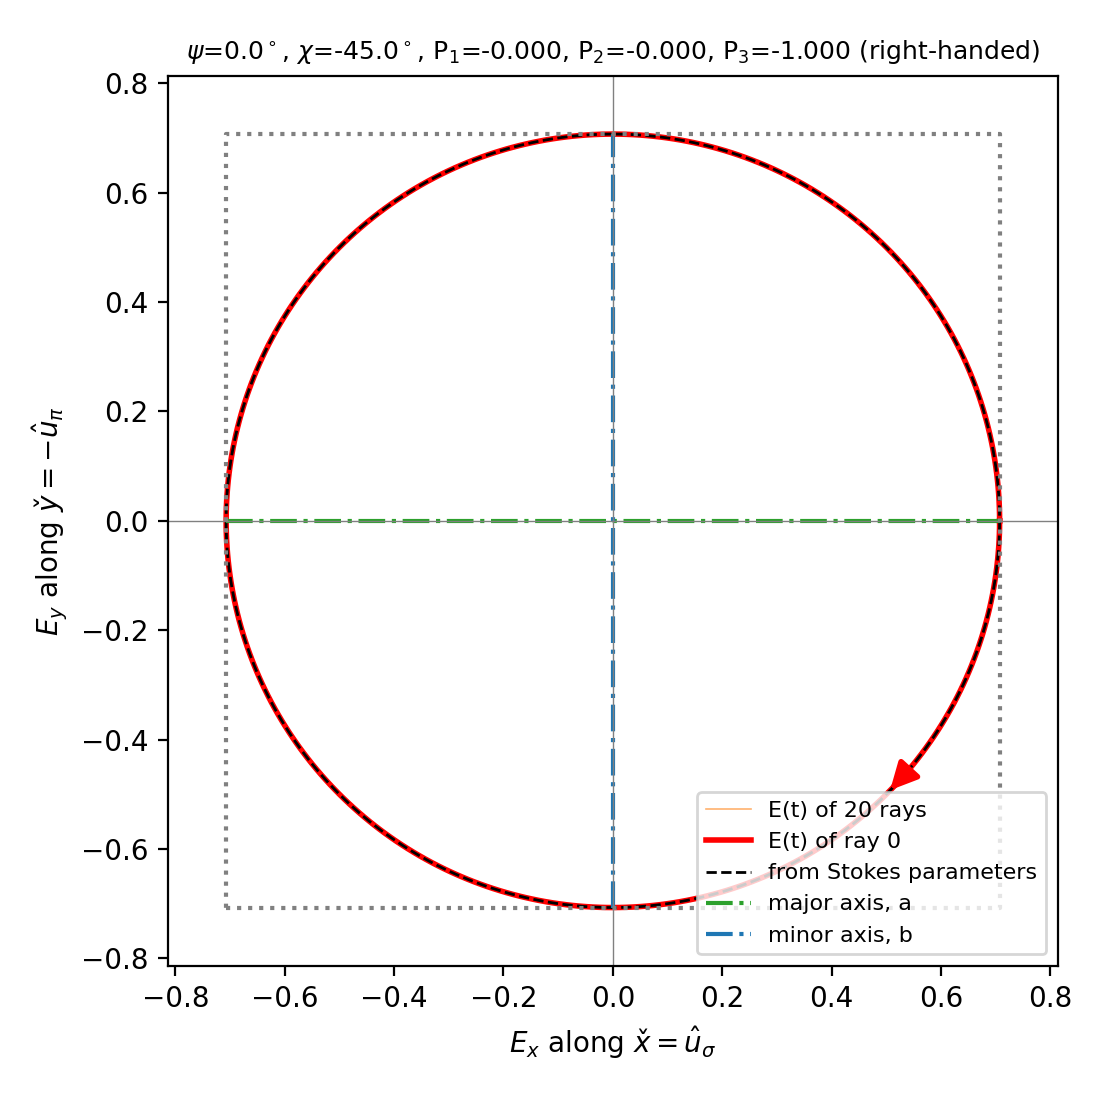
\includegraphics[width=0.85\linewidth]{figures/polarization_ellipse_geometrical_rcp.png}\\
(a)\\
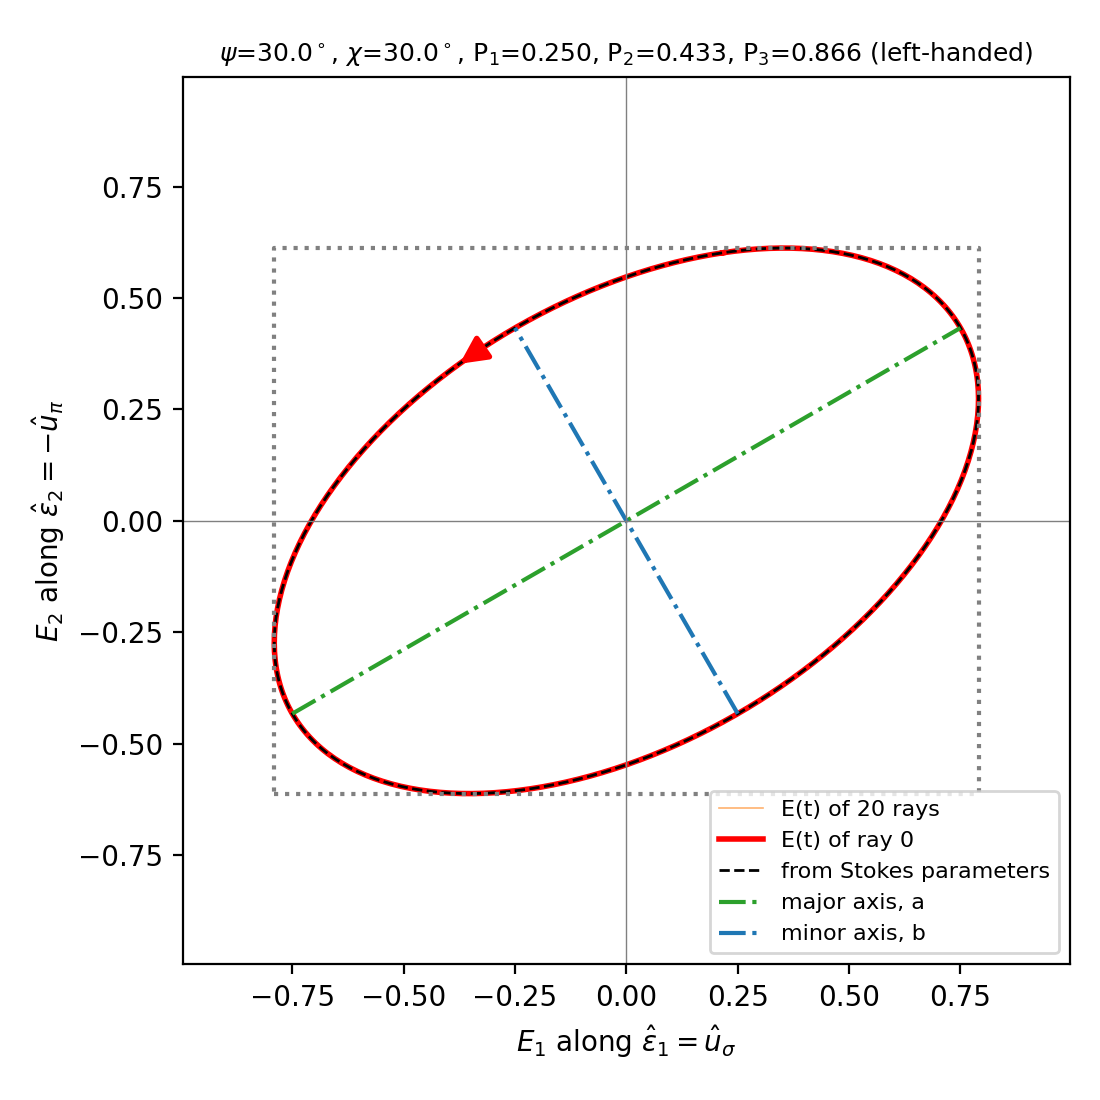
\includegraphics[width=0.85\linewidth]{figures/polarization_ellipse_geometrical.png}\\
(b)
\caption{Polarization ellipses of beams from a geometrical source, seen by an observer looking toward the source: (a) $P=0.5$ and $\Phi=90^\circ$ (right circular polarization, $\chi=-45^\circ$); (b) $P=0.5635$ and $\Phi=-116.57^\circ$ ($\psi=\chi=30^\circ$, left-handed elliptical polarization). The electric field of a sample of 20 rays (thin lines), and of one of them (thick line, with the arrow indicating the sense of rotation), coincide with the ellipse obtained from the Stokes parameters of the beam (dashed line), with its major and minor axes (for circular polarization, $\psi$ is undefined and set to zero). The dotted rectangle has sides $2|E_x|$ and $2|E_y|$.}
\label{fig:ellipse_geometrical}
\end{figure}

\subsection{Polarization of a bending magnet source}\label{sec:source_bm}
\label{sec:polarization_bm}

In a bending magnet source the polarization of each ray depends on its emission direction. SHADOW samples the ray directions and energies from the synchrotron emission \cite{SanchezdelRio2024bm}, and sets the amplitudes of the $\sigma$ and $\pi$ components (horizontal and vertical, respectively) from the emission functions of the two polarizations at the vertical angle of the ray. The radiation is linearly polarized in the plane of the orbit, and elliptically polarized out of it, with phase difference $\Phi=\pm 90^\circ$ (the sign changes with the sign of the vertical angle), therefore with opposite handedness above and below the orbit plane.

Fig.~\ref{fig:ellipse_bm} shows the polarization ellipses for a bending magnet of the old ESRF storage ring (electron energy 6.04~GeV, magnetic field $B=-0.8$~T, radius 25.18~m, critical energy 19.4~keV), the same source used in \cite{SanchezdelRio2024bm}, at the photon energy of 8~keV. Every ray is fully polarized, but the ellipses of the rays are different: from nearly linear horizontal polarization (rays close to the orbit plane) to elliptical polarization with a large vertical component and either handedness (rays at larger vertical angles). All ellipses have their axes along $\check{x}$ and $\check{y}$ ($\Phi=\pm90^\circ$).
The Stokes parameters of the beam (5000 rays) are $P_1=0.674$, $P_2=0.000$ and $P_3=-0.014$: the contributions of the two handednesses cancel ($P_3\approx 0$ for a beam symmetric with respect to the orbit plane), and the beam is partially polarized, with DOP=0.674, although every ray is fully polarized. The ellipse of the polarized part degenerates to a horizontal line: the polarized part of the beam is linearly polarized in the orbit plane.

\begin{figure}
\centering
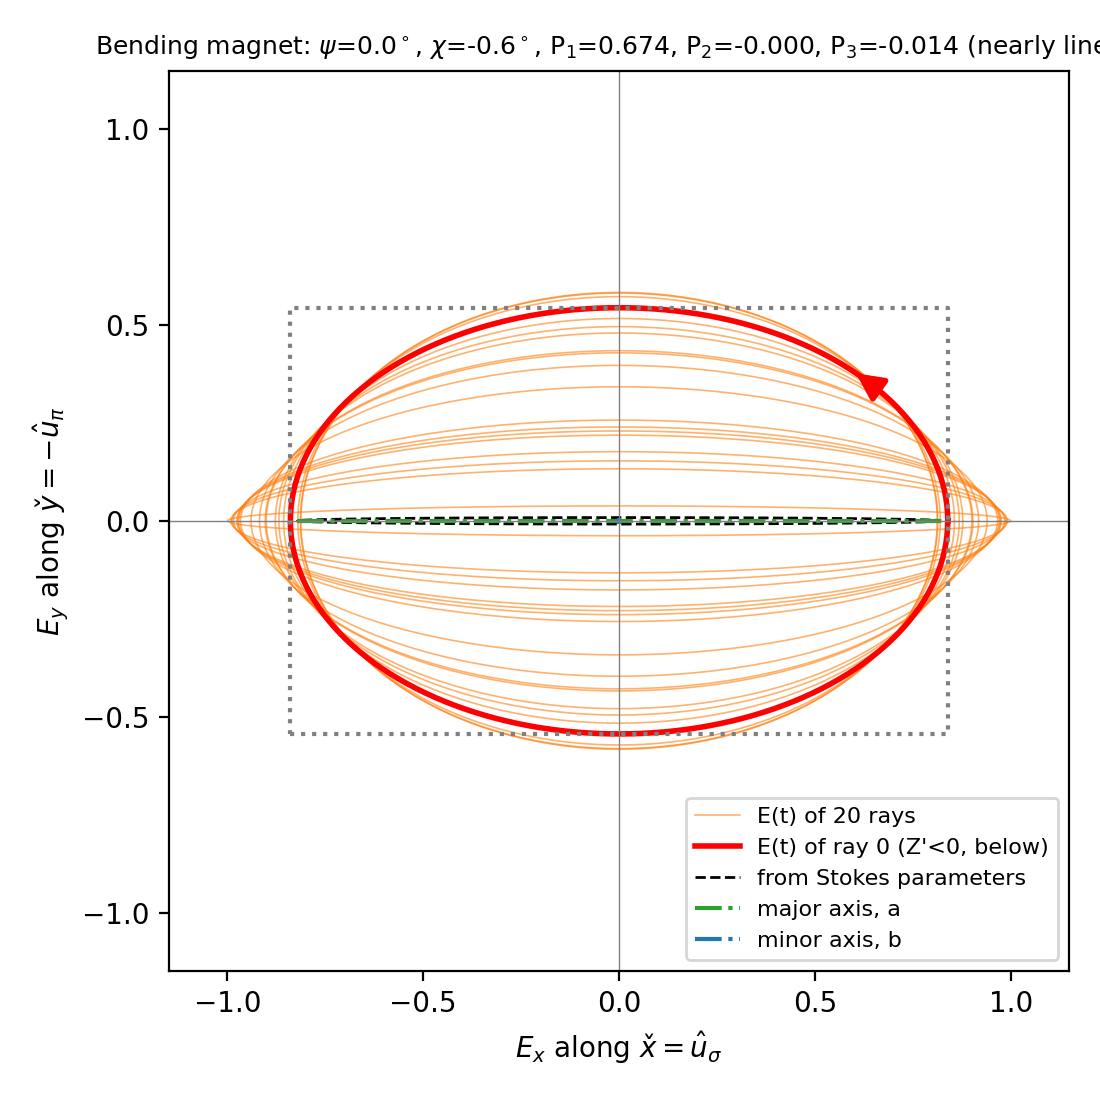
\includegraphics[width=0.85\linewidth]{figures/polarization_ellipse_bending_magnet.png}
\caption{Polarization ellipses for an ESRF bending magnet (6.04~GeV, 0.8~T) at 8~keV, seen by an observer looking toward the source: electric field of a sample of 20 rays (thin lines) and of one of them (thick line, the arrow indicates the sense of rotation), emitted below the orbit plane ($Z'=-97~\mu$rad) and therefore left-handed (counter-clockwise). The ellipse of the polarized part of the beam, obtained from the summed Stokes parameters (dashed line), degenerates to a horizontal line (DOP=0.674).}
\label{fig:ellipse_bm}
\end{figure}

Fig.~\ref{fig:bm_stokes} shows the Stokes parameters of the rays versus their vertical direction $Z'$ (column 6), for the same source without electron beam emittance, so that $Z'$ is the emission angle $\psi_v$. The normalized Stokes parameters of every ray coincide (to $4\times10^{-6}$) with the expressions of the synchrotron radiation \cite{Jackson1999,xraydatabooklet}, $\mathcal{E}_\sigma\propto(1+X^2)K_{2/3}(\xi)$ and $|\mathcal{E}_\pi|\propto|X|(1+X^2)^{1/2}K_{1/3}(\xi)$, with $X=\gamma\psi_v$, $\xi=(E/2E_c)(1+X^2)^{3/2}$, and a phase difference of $\pm90^\circ$. $P_1$ decreases from 1 in the orbit plane, $P_2=0$, and $|P_3|$ increases with $|Z'|$, reaching $|P_3|\approx1$ in the tails of the angular distribution, where the intensity is small. The sign of $P_3$ changes with the sign of $Z'$. In this example ($B<0$), the electrons are deflected toward $+\hat{x}$, i.e., they turn clockwise seen from above, and the radiation emitted above the orbit plane ($Z'>0$) is right-handed ($S_3<0$), and below it left-handed ($S_3>0$). The averages are $P_3=-0.637$ for the rays above and $+0.638$ for the rays below the orbit plane, while $P_3\approx0$ for the whole beam. This agrees with the literature, where the radiation emitted upward has negative helicity (RCP, $S_3<0$) when the electrons travel clockwise seen from above \cite{Schafers2008}, and with a direct calculation of the Li\'enard--Wiechert field of an electron on the same orbit, which shows that the electric field above the orbit plane rotates clockwise for an observer looking toward the source. For electrons travelling counter-clockwise, the handedness is reversed. A beam with circular polarization of a given handedness can therefore be obtained by selecting with a slit the rays above or below the orbit plane, at the expense of intensity. In SHADOW4 the handedness is set by the sign of the magnetic field, i.e., by the sense of rotation of the electrons.

\begin{figure}
\centering
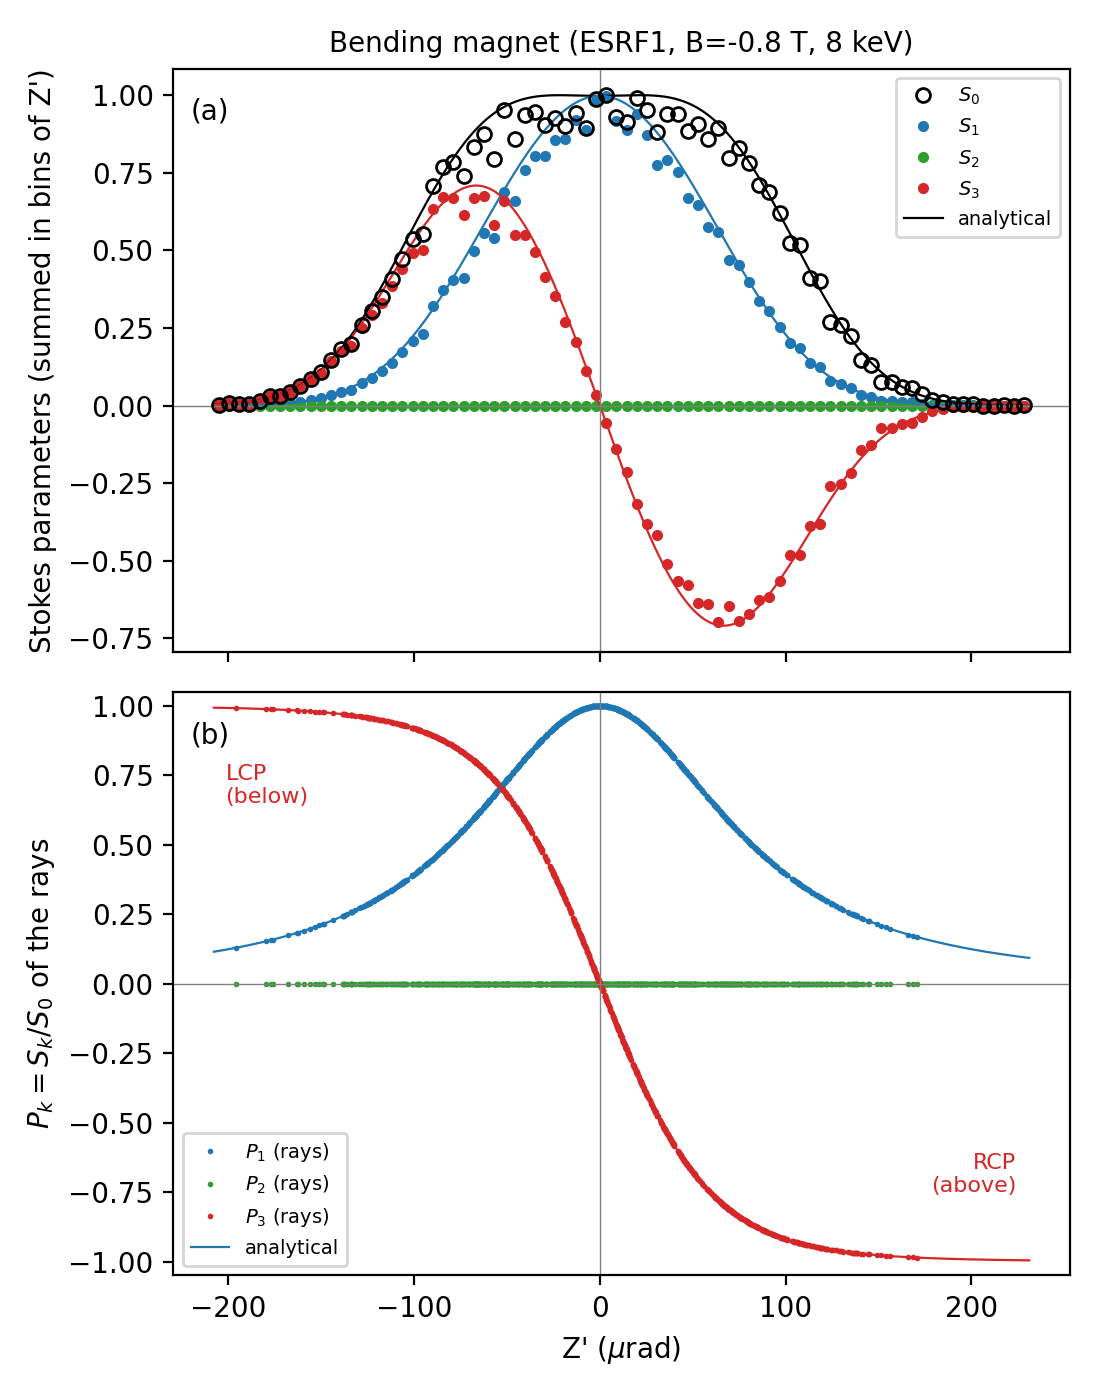
\includegraphics[width=0.85\linewidth]{figures/stokes_bending_magnet.png}
\caption{Stokes parameters of the rays of an ESRF bending magnet (6.04~GeV, $B=-0.8$~T, electrons turning clockwise seen from above) at 8~keV versus the vertical direction $Z'$ of the rays: (a) Stokes parameters summed in bins of $Z'$ (normalized to the maximum of $S_0$), and (b) normalized Stokes parameters $P_k=S_k/S_0$ of the rays (one in twenty is plotted). The lines are the analytical expressions. The radiation is right-handed ($S_3<0$) above and left-handed ($S_3>0$) below the orbit plane.}
\label{fig:bm_stokes}
\end{figure}

% -----------------------------------------------------------------
% -----------------------------------------------------------------
\section{Interaction with the optical elements}\label{sec:interaction}
% -----------------------------------------------------------------
% -----------------------------------------------------------------

The interaction of the rays with an optical element is done in three steps: the rays are expressed in the reference frame of the element (section~\ref{sec:change_frame}), the scattering by the element changes their direction and electric field (section~\ref{sec:S4}), and they are expressed in the reference frame of the image plane.

\subsection{Reference frames and orientation of the element}\label{sec:change_frame}
SHADOW uses local reference systems associated to the source and image planes and to the beamline elements (see Fig.~\ref{fig:S4_reference_frame}).
This allows iterating over the beamline elements: each one has two ``continuation planes'': the source and the image.

In SHADOW4 the ``beamline element'' is formed by an ``optical element'' object and a ``coordinates'' object containing three angles: the incidence angle $\theta$ and the exit angle $\theta'$ (both measured from the normal to the surface; they differ for gratings and asymmetric crystals), and the beamline element orientation angle $\alpha$; and two distances: the distance $p$ from the source (or continuation plane from the previous element), and $q$ from the beamline element to its image plane or continuation plane.
The beamline element orientation angle $\alpha$ is not reset after the scattering in the beamline element (reflection, refraction or diffraction), therefore it influences the orientation of the axis at the image (see Fig.~\ref{fig:S4_orientations}).

\begin{figure}
    \centering
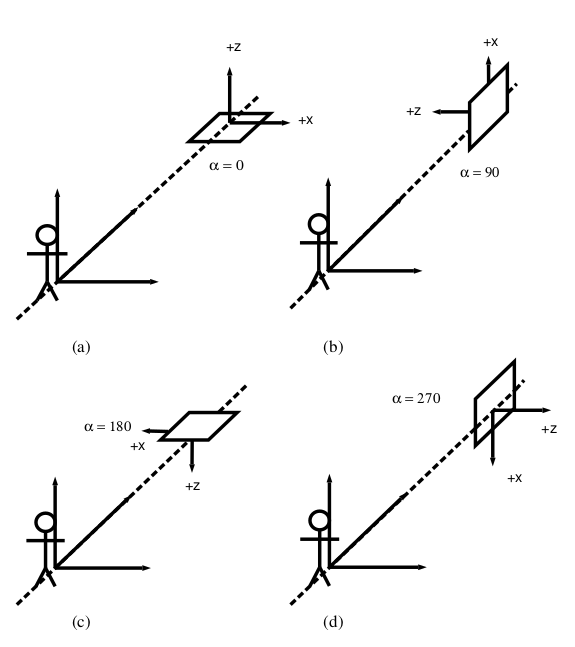
\includegraphics[width=0.9\linewidth]{figures/S4_orientations.png}
\caption{Effect of the beamline element orientation angle $\alpha$ for the four most common values: 0, 90, 180 and 270 degrees. The effect of the angle $\alpha$ is carried over to the image plane, thus defining the position of the axes (in blue). }
\label{fig:S4_orientations}
\end{figure}


The beam coming from the source or a previous beamline element must be converted into the reference frame of the beamline element for performing the ray tracing.
This is done with the method {\tt S4Beam.rotate}\footnote{\tiny \url{https://shadow4.readthedocs.io/en/latest/shadow4.beam.html#shadow4.beam.s4_beam.S4Beam.rotate}}, which is a change of coordinates: all the vectors of the rays ($\vec{x}$, $\vec{v}$ and $\vec{E}_{\sigma,\pi}$) are re-expressed in a set of axes rotated by a given angle around a given axis.
To put the beam in the local reference of the beamline element, these sequential operations are applied:
\begin{itemize}
    \item rotate the axes by the angle $\alpha$ around $\hat{u}_y$=(0,1,0) (from $x$ toward $z$);
    \item rotate the axes by the grazing angle $\theta_g=\pi/2-\theta$ around $\hat{u}_x$=(1,0,0);
    \item translate the beam coordinates $\vec{r}$ a distance $p$ backwards along the incident direction, i.e., by $(0, -p\cos\theta_g, p\sin\theta_g)$.
\end{itemize}
As an example, see the listed code\footnote{\tiny \url{https://shadow4.readthedocs.io/en/latest/shadow4.beamline.optical_elements.mirrors.html#shadow4.beamline.optical_elements.mirrors.s4_mirror.S4MirrorElement.trace_beam}}.
For a ray along the axis of the beamline element, the first rotation turns the $\sigma$ direction of the ray by $\alpha$ with respect to the $\sigma$ direction of the beamline element, so $\alpha$ is the angle used in the Jones rotation matrix of section~\ref{sec:S4} [equation~(\ref{eq:rotation})].
If movements (offsets or rotations) of the beamline element are defined, they are applied after these operations, and undone after the interaction.

Then, the reflection/refraction/diffraction by the beamline element is applied, which changes the beam direction and electric vectors.
This is discussed in section~\ref{sec:S4}.

Last, after the interaction with the beamline element, the rays are\footnote{
These operations are done by the method {\tt S4Beam.change\_to\_image\_reference\_system}, see: {\tiny \url{https://shadow4.readthedocs.io/en/latest/shadow4.beam.html#shadow4.beam.s4_beam.S4Beam.change_to_image_reference_system}}.
}
\begin{itemize}
    \item propagated along their directions up to the image plane, which is perpendicular to the central outgoing ray at a distance $q$ (the outgoing grazing angle $\pi/2-\theta'$ is used), and
    \item expressed in the image coordinate system, with origin at the center of the image plane. For that, all the vectors ($\vec{r}$, $\vec{v}$ and $\vec{E}_{\sigma,\pi}$) are projected onto the versors of the new reference.
\end{itemize}
The optical path is increased by the propagated distance (times the refraction index).

It is important that the changes of reference system (before and after interaction with the beamline element) do not affect the phases $\phi_\sigma$ and $\phi_\pi$, and conserve the modulus of each electric field component $\vec{E}_\sigma$ and $\vec{E}_\pi$. Being rotations, they also conserve the Stokes parameters of the rays, and do not alter the orthogonality relationships:
\begin{eqnarray}
\label{ortho}
\vec{E}_\sigma \perp \vec{E}_\pi \nonumber \\
\vec{E}_\sigma \perp \vec{v} \nonumber \\
\vec{E}_\pi \perp \vec{v}.
\end{eqnarray}

\subsection{Jones calculus in the scattering plane}\label{sec:S4}

The interaction of the SHADOW beam with the optical element  uses the Jones calculus \cite{Jones1941a, Jones1941b} in SHADOW4. We explain here the theory and implementation. This is new in SHADOW4, and the old implementation in SHADOW3 is described in Appendix~\ref{sec:S3}.

Fully polarized light can be described using the Jones calculus. The polarized electric field is represented by a Jones vector, made by two complex numbers representing the scalar electric field for the $\sigma$ and $\pi$ polarizations. 
The effect of the beamline elements is represented by Jones matrices.
In such a way, the light after the interaction with the optical element is found by taking the product of the Jones matrix of the optical element and the Jones vector of the incident light.

The Jones vector of a ray, following equation~(\ref{eq:electricfieldray2}), is
\begin{equation}
        \begin{pmatrix}
        \mathcal{E}_\sigma \\
        \mathcal{E}_\pi
    \end{pmatrix}
    =
    \begin{pmatrix}
        |\vec{E}_{\sigma}| e^{i \phi_\sigma} \\
        |\vec{E}_{\pi}| e^{i \phi_\pi}
    \end{pmatrix}.
\end{equation}
This Jones vector is expressed in the SHADOW basis $(\hat{u}_\sigma,\hat{u}_\pi,\vec{v})$, which is left-handed (section~\ref{sec:handedness}); the standard Jones vector, $(\mathcal{E}_\sigma,-\mathcal{E}_\pi)^T$, is used only to compute the Stokes parameters and the polarization ellipse. The physics does not depend on this choice: a Jones matrix $\textbf{J}_{std}$ defined in the standard basis is written in the SHADOW basis as $\textbf{F}\cdot\textbf{J}_{std}\cdot\textbf{F}$, with $\textbf{F}=\mathrm{diag}(1,-1)$. For a diagonal matrix, as for mirrors and crystals, the two are identical; for non-diagonal elements, the off-diagonal elements change sign (this conversion is done in SHADOW4 by {\tt S4Beam.jones\_matrix\_standard\_to\_shadow}).

In general, a Jones matrix is applied to a Jones vector to get the scattered Jones vector
\begin{equation}\label{eq:applyJones}
    \begin{pmatrix}
        \mathcal{E}'_\sigma \\
        \mathcal{E}'_\pi
    \end{pmatrix}
    =
    \textbf{J}
    \cdot
    \begin{pmatrix}
        \mathcal{E}_\sigma\\
        \mathcal{E}_\pi
    \end{pmatrix}.
\end{equation}

The Jones matrix that represents a generic beamline element is\footnote{The off-diagonal elements in the most common beamline elements like crystals, gratings, mirrors and multilayer are zero}
\begin{equation}\label{eq:J}
\textbf{J}_e = 
\begin{pmatrix}
r_{\sigma\sigma} & r_{\sigma\pi}\\
r_{\pi\sigma} & r_{\pi\pi}
\end{pmatrix},
\end{equation}
where the elements are the complex scattering amplitudes.
Note that the $\sigma$ and $\pi$ directions here are ``local'' (they are referred to the scattering plane).
This implies that $\textbf{J}_e$ in equation~(\ref{eq:J}) cannot be directly applied to the Jones vector of the incident ray, but has to be transformed. 

The $\sigma$ and $\pi$ directions of polarization are defined by the scattering plane spanned by the direction vectors before and after the scattering: $\vec{v}$ and $\vec{v}'$, respectively.
It is convenient to consider the $\sigma$ and $\pi$ versors in three different frames, all following the SHADOW convention of equation~(\ref{eq:upi}), i.e., $\hat{u}_\pi = \hat{u}_\sigma \times$ (ray direction), so that every triad $(\hat{u}_\sigma, \hat{u}_\pi, \text{ray direction})$ is left-handed [equation~(\ref{eq:lefthanded})]:
\begin{itemize}
    \item the $\hat{u}_\sigma$ and $\hat{u}_\pi$ for the incoming ray as defined in equation~(\ref{eq:electricfieldray2}), 

    \item for the scattering plane spanned by $\vec{v}$ (incident direction): 

\begin{eqnarray}\label{eq:u_i}
  \hat{u}_{\sigma,i} 
  &=&
  \frac{\vec{v} \times \vec{v}'}{\left| \vec{v} \times \vec{v}' \right|}
  \nonumber \\
  \hat{u}_{\pi,i}
  &=&
  \frac{\hat{u}_{\sigma,i} \times \vec{v}}{\left| \hat{u}_{\sigma,i} \times \vec{v} \right|}.
\end{eqnarray}

    \item for the scattering plane spanned by $\vec{v}'$ (output or final direction): 

\begin{eqnarray}\label{eq:u_f}
  \hat{u}_{\sigma,f} 
  &=&
  \hat{u}_{\sigma,i} 
  \nonumber \\
  \hat{u}_{\pi,f}
  &=&
  \frac{\hat{u}_{\sigma,f} \times \vec{v}'}{\left| \hat{u}_{\sigma,f} \times \vec{v}' \right|}.
\end{eqnarray}
\end{itemize}
All $\hat{u}$ are real 3D unit vectors.
With this choice, $\hat{u}_{\pi,i}\cdot\hat{u}_{\pi,f} = \vec{v}\cdot\vec{v}' = \cos\Theta$, with $\Theta$ the scattering angle (e.g., $\Theta=2\theta_g$ for a mirror with grazing angle $\theta_g$, or $\Theta=2\theta_B$ for a symmetric Bragg reflection), which is the usual polarization factor of the $\pi$ component.
Note that in forward scattering, $\vec{v}' = \vec{v}$, the scattering plane is ill defined, and an arbitrary direction can be chosen: we use $\hat{u}_{\sigma,i}=\hat{u}_{\sigma}$, therefore $\hat{u}_{\pi,i}=\hat{u}_{\pi}$ and $\textbf{R}$ is the identity.

The electric vector in the frame related to the diffraction plane (with axes along $\hat{u}_{\sigma,i}$, $\vec{v}$, and $\hat{u}_{\pi,i}$) is expressed as 
\begin{equation}
  \left( \begin{array}{c}
    E_{\sigma,i} e^{i \phi_{\sigma,i}} \\
    E_{\pi,i} e^{i \phi_{\pi,i}}
  \end{array} \right)
  =
  \underbrace{
  \left( \begin{array}{cc}
    \hat{u}_{\sigma,i} \cdot \hat{u}_{\sigma} &
    \hat{u}_{\sigma,i} \cdot \hat{u}_{\pi} \\
    \hat{u}_{\pi,i} \cdot \hat{u}_{\sigma} &
    \hat{u}_{\pi,i} \cdot \hat{u}_{\pi} 
  \end{array} \right)
  }_{\textbf{R}(\alpha)}
  \cdot
  \left( \begin{array}{c}
    E_{\sigma} e^{i \phi_{\sigma}} \\
    E_{\pi} e^{i \phi_{\pi}}
  \end{array} \right).
\end{equation}

The $2\times 2$ matrix is a coordinate transform (a ``passive'' rotation: the field is fixed and the axes are rotated). Let $\alpha$ be the angle from $\hat{u}_\sigma$ to $\hat{u}_{\sigma,i}$, measured toward $\hat{u}_\pi$, i.e., $\hat{u}_{\sigma,i}=\cos\alpha~\hat{u}_\sigma + \sin\alpha~\hat{u}_\pi$. Using equation~(\ref{eq:u_i}) and $\hat{u}_\pi \times \vec{v} = -\hat{u}_\sigma$, it follows $\hat{u}_{\pi,i}=-\sin\alpha~\hat{u}_\sigma + \cos\alpha~\hat{u}_\pi$, and

\begin{equation}\label{eq:rotation}
  \textbf{R}(\alpha)
  =
  \left( \begin{array}{cc}
    \cos(\alpha) & \sin(\alpha) \\
    -\sin(\alpha) & \cos(\alpha)
 \end{array} \right).
\end{equation}
For a ray along the axis of the beamline element, $\alpha$ coincides with the orientation angle of the beamline element (section~\ref{sec:change_frame}).
Note that, because the triad $(\hat{u}_\sigma, \hat{u}_\pi, \vec{v})$ is left-handed, a positive $\alpha$ corresponds to a clockwise rotation for an observer looking toward the source.
The transpose of $\textbf{R}(\alpha)$ [i.e., $\textbf{R}(-\alpha)$, the ``active'' rotation matrix] must not be used here: it gives the same result only for $\alpha$ multiple of $90^\circ$ (for $\alpha=\pm 90^\circ$ the two matrices differ only in a global sign).


% The $\sigma$ direction is coincident with the $x$ axis when the surface normal is along $z$ and the scattering plane is $yz$ (this is the default case). The $\pi$ direction is therefore in the $yz$ plane, and is perpendicular to $\sigma$ and the incident direction $\vec{v}$.

% https://pleclair.ua.edu/optics/Notes/Jones.pdf

% A rotation matrix in 2D transforms the coordinates of a generic point $(x_1,x_2)^T$ into the coordinates $(x'_1,x'_2)^T$ in a new reference system rotated an angle $\phi$ is (see, e.g., \cite{LeClair})
% \begin{equation}
% \textbf{R}(\phi) = 
% \begin{pmatrix}
% \cos\phi & -\sin\phi\\
% \sin\phi & \cos\phi
% \end{pmatrix},
% \end{equation}
% in such a way that
% \begin{equation}
% \begin{pmatrix}
% x'_1 \\
% x'_2
% \end{pmatrix} = 
% \textbf{R}(\phi)
% \begin{pmatrix}
% x_1 \\
% x_2
% \end{pmatrix}.
% \end{equation}

The Jones matrix in equation~(\ref{eq:J}) is now applied to the incident Jones vectors as

\begin{equation}\label{eq:JR}
  \left( \begin{array}{c}
    \mathcal{E}_{\sigma,f} \\
    \mathcal{E}_{\pi,f}
  \end{array} \right)
  =
    \textbf{J}_e \cdot
  \left( \begin{array}{c}
    \mathcal{E}_{\sigma,i} \\
    \mathcal{E}_{\pi,i}
  \end{array} \right)
  =
  \textbf{J}_e \cdot \textbf{R}(\alpha) \cdot
  \left( \begin{array}{c}
    E_{\sigma} e^{i \phi_{\sigma}} \\
    E_{\pi} e^{i \phi_{\pi}}
  \end{array} \right),
\end{equation}
where $\mathcal{E}$ are complex amplitudes along the different direction versors.

% Consider now an incident ray whose electric fields is along the directions $\vec{u}_\sigma$ and $\vec{u}_\pi$. Let be $\alpha$ the angle between $\vec{u}_\sigma$ and $\sigma$ direction of the beamline element  (always perpendicular to the scattering plane). The Jones matrix to be applied to this ray is\footnote{
% In \cite{LeClair} it is said that if an optical element is rotated about the optical axis by an angle $\alpha$, the Jones matrix for the
% rotated element $\textbf{J}_\alpha$ is constructed from the matrix for the unrotated element $\textbf{J}$ by rotating by an angle $\alpha$, applying the matrix $\textbf{J}$, and rotating back by an angle $\-\alpha$:
% $\textbf{J}_\alpha = \textbf{R}(-\alpha) \textbf{J} \textbf{R}(\alpha)$.
% Considering that in SHADOW the rotation of $\alpha$ is not reset, it implies that we must use instead the equation~(\ref{eq:Jalpha_S4}).
% }
% \begin{equation}\label{eq:Jalpha_S4}
%     \textbf{J}_\alpha =  \textbf{J} \textbf{R}(\alpha)=
%     \begin{pmatrix}
% r_\sigma c & -r_\sigma s\\
% r_\pi s& 
% r_\pi c
% \end{pmatrix}.
% \end{equation}
% Therefore, the particular cases for zero and 90$^\circ$ are
% \begin{equation}
% \textbf{J}_{0^\circ} = 
% \begin{pmatrix}
% r_\sigma & 0\\
% 0 & r_\pi
% \end{pmatrix},\text{~and~}
% \textbf{J}_{90^\circ} = 
% \begin{pmatrix}
% 0 & -r_\sigma\\
% r_\pi & 0
% \end{pmatrix}. \nonumber
% \end{equation}
%
% Jones vector $E^J$ for a ray, following Eq.~\ref{eq:electricfieldray}, is
% \begin{equation}
%     E^J = 
%         \begin{pmatrix}
%         e_1 \\
%         e_2
%     \end{pmatrix}
%     =
%     \begin{pmatrix}
%         |E_{\sigma}| e^{i \phi_\sigma} \\
%         |E_{\pi}| e^{i \phi_\pi}
%     \end{pmatrix}.
% \end{equation}

To convert a Jones vector to SHADOW variables we must know the versors with the directions of the electric field.
After scattering of a beamline element, the versors to consider are those of equations~(\ref{eq:u_f}).
Then, $\vec{E}_\sigma=|\mathcal{E}_\sigma| \hat{u}_{\sigma,f}$, and 
$\phi_\sigma=\arg(\mathcal{E}_{\sigma,f})$
(and a similar expression holds for the $\pi$ component).

Note that in the SHADOW description the vectors $\vec{E}_{\sigma,\pi}$ and the phases $\phi_{\sigma,\pi}$ are not independent: a change of sign of $\vec{E}_\sigma$ is equivalent to adding $\pi$ to $\phi_\sigma$ (same for $\pi$). Also, multiplying both components of the Jones vector by a common phase factor $e^{-i\phi_\sigma}$, i.e., setting $\phi_\pi \xleftarrow{}(\phi_\pi-\phi_\sigma)$ and $\phi_\sigma\xleftarrow{}0$ without changing the vectors $\vec{E}_{\sigma,\pi}$, gives the same polarization state and intensity of the ray. However, this global phase is not irrelevant for coherent beams, where it determines the interference between rays, and it is not modified by SHADOW4.


% In SHADOW4 we calculate the scattering in a beamline element (mirror and multilayer reflections, crystal and grating diffraction, lens refraction) applying the Jones formalist.

In summary, the different steps to be followed in the ray-tracing calculation, considering the input beam already in the local reference of the beamline element (i.e., all the vectors such as direction and electric fields are expressed in the optical element local reference, as described in section~\ref{sec:change_frame}), are:

\begin{enumerate}

\item From every ray we extract the input direction $\vec{v}$, the phases $\phi_{\sigma,\pi}$, and the electric field vectors $\vec{E}_{\sigma,\pi}$. We construct the versor directions $\hat{u}_{\sigma,\pi}$, and the Jones vector $(\mathcal{E}_\sigma, \mathcal{E}_\pi)^T$.

\item From the model of the beamline element we obtain the outgoing direction $\vec{v}'$ (geometrical model), and the reflectivities (physical model) to build $\mathbf{J}_e$ [equation~(\ref{eq:J})].

\item Construct the versors in equations~(\ref{eq:u_i}) and (\ref{eq:u_f}) and the matrix $\textbf{R}(\alpha)$.


\item Compute the Jones matrix $\textbf{J}_e \cdot \textbf{R}(\alpha)$ [equations~(\ref{eq:J}) and (\ref{eq:rotation})].

\item Calculate the scattered Jones vector $(\mathcal{E}_{\sigma,f}, \mathcal{E}_{\pi,f})^T$ using equation~(\ref{eq:JR}).

\item Compute the SHADOW variables $\vec{E}'_{\sigma,\pi}$ and $\phi'_{\sigma,\pi}$ for the scattered ray with the amplitudes in the scattered Jones vector and the directions $\hat{u}_{\sigma,f}$ and $\hat{u}_{\pi,f}$.
\end{enumerate}

%################################

\subsection{Forward scattering: the transmitted beam}\label{sec:forward}

In the transmitted (forward-diffracted) beam of a crystal, the outgoing direction coincides with the incident one, but the polarization is changed. Its amplitudes $t_\sigma$ and $t_\pi$ are given in Appendix~\ref{sec:mirrorandcrystals} [equation~(\ref{eq:tbragg})].
For the transmitted beam, the incident and outgoing directions coincide ($\vec{v}'=\vec{v}$), and the scattering plane defined in section~\ref{sec:S4} is not defined. However, the $\sigma$ and $\pi$ directions of $t_\sigma$ and $t_\pi$ are those of the diffraction plane, spanned by $\mathbf{k}_0$ and $\mathbf{k}_h$. Therefore, the Jones matrix $\textbf{J}_e=\mathrm{diag}(t_\sigma,t_\pi)$ of a transmitting crystal must be applied using $\hat{u}_{\sigma,i}=\hat{u}_{\sigma,f}=\mathbf{k}_0\times\mathbf{k}_h/|\mathbf{k}_0\times\mathbf{k}_h|$ in equations~(\ref{eq:u_i}) and (\ref{eq:u_f}) [with $\hat{u}_{\pi,i}=\hat{u}_{\pi,f}=\hat{u}_{\sigma,i}\times\vec{v}$], and not with the arbitrary choice used above for forward scattering, which is only valid when $t_\sigma=t_\pi$.

\subsection{Equivalent configurations: rotating the polarization or the element}\label{sec:equivalence}

In equation~(\ref{eq:JR}), the incident field enters the interaction only through its components $\textbf{R}(\alpha)\cdot(\mathcal{E}_\sigma,\mathcal{E}_\pi)^T$ in the $\sigma$ and $\pi$ directions of the scattering plane. Therefore, two configurations that give the same components are physically equivalent. For example, a ray with horizontal linear polarization [$P=1$, Jones vector $(1,0)^T$] incident on an element rotated by $\alpha=-45^\circ$ has the components $\textbf{R}(-45^\circ)\cdot(1,0)^T=(1,1)^T/\sqrt{2}$, the same as a ray linearly polarized at $45^\circ$ [$P=0.5$, $\Phi=0$, Jones vector $(1,1)^T/\sqrt{2}$, i.e., electric field along $\hat{u}_\sigma+\hat{u}_\pi$] incident on the element with $\alpha=0$. The outgoing rays are identical, including their Stokes parameters, which refer to the $\sigma$ direction of the outgoing ray. With $\alpha=+45^\circ$ the components are $(1,-1)^T/\sqrt{2}$: this is the mirror-symmetric configuration, which reverses the signs of $P_2$ and $P_3$ (and therefore the handedness of a circular polarization), but not of $P_1$.
This equivalence is used to check SHADOW4 in the examples of sections~\ref{sec:polarizers_all} and \ref{sec:phaseshifters_all}. Note that it holds ray by ray only if the incidence angle on the element is the same in both configurations, e.g., for pencil beams, or for a divergence contained in the plane of incidence of the element.


% -----------------------------------------------------------------
% -----------------------------------------------------------------
\section{Polarizers}\label{sec:polarizers_all}
% -----------------------------------------------------------------
% -----------------------------------------------------------------

A polarizer transmits (or reflects) one linear polarization and suppresses the orthogonal one. We first consider the simplest case, the reflection of visible light by a glass surface at the Brewster angle, which can be compared with the Fresnel equations, and then the X-ray polarizers made of crystals with a Bragg angle close to $45^\circ$.

\subsection{Visible range: mirrors at the Brewster angle}\label{sec:visible_polarizers}
Polarizing light using mirror reflection exploits the phenomenon of Brewster's angle. The Brewster angle emerges naturally from the Fresnel equations \cite{born_wolf}, which describe the reflection and transmission of light at the interface between two media. At the Brewster angle, the reflection coefficient for $\pi$-polarized light becomes zero, leading to complete transmission of the $\pi$-polarized component into the second medium. This phenomenon results in the reflected light being completely $\sigma$-polarized.

To check this, we created in SHADOW4 a pencil beam (point source, zero divergence and monochromatic), where all rays are identical, with horizontal linear polarization ($P=1$, $\Phi=0$). We send the beam to a plane glass mirror (refraction index $n$=1.51) rotated azimuthally by $\alpha=-45^\circ$, and we scan the incident angle (each point comes from a different SHADOW4 run). The intensities of the $\sigma$ and $\pi$ components of the reflected ray versus the incident angle are shown in Fig.~\ref{fig:visible}(a). As the incident ray has equal $\sigma$ and $\pi$ intensities (0.5 each) with respect to the scattering plane of the mirror, these intensities are $|r_s|^2/2$ and $|r_p|^2/2$, which compare directly with the reflectances in Fig. 1.12 of \cite{born_wolf} (6th edition). The intensity of the $\pi$ component vanishes at the Brewster angle $\theta_{Bw}=\arctan(1.51)=56.5^\circ$.
As expected (section~\ref{sec:equivalence}), the same results are obtained with a beam linearly polarized at $45^\circ$ ($P=0.5$, $\Phi=0$) and the mirror at $\alpha=0$ (Fig.~\ref{fig:visible}).
%Note that the orientation angle must be $-45^\circ$: with $\alpha=+45^\circ$ the intensities are the same, but the phase difference changes by $\pi$, because then the field corresponds to $P=0.5$ and $\Phi=180^\circ$ (along $\hat{u}_\sigma-\hat{u}_\pi$).
The change of phase ($\sigma$ minus $\pi$) is $\pi$ below the Brewster angle, and zero above it (Fig.~\ref{fig:visible}(b)).

\begin{figure}
\centering
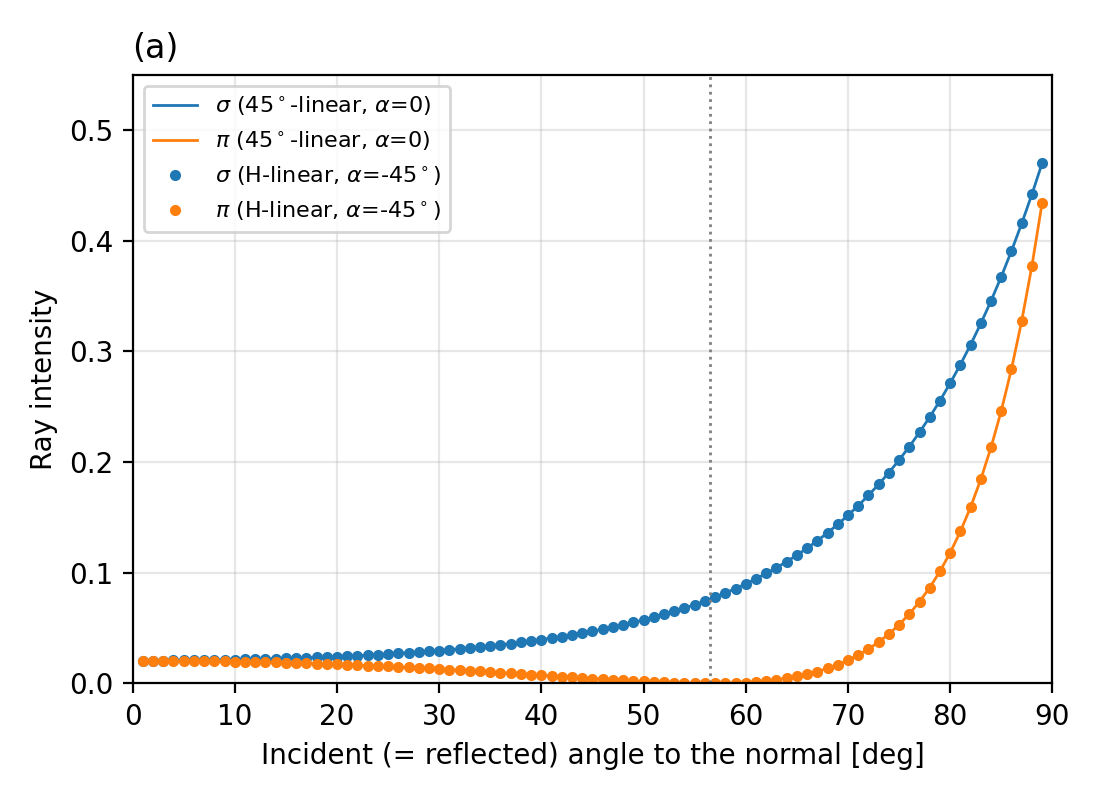
\includegraphics[width=0.95\linewidth]{figures/visibleR.png}
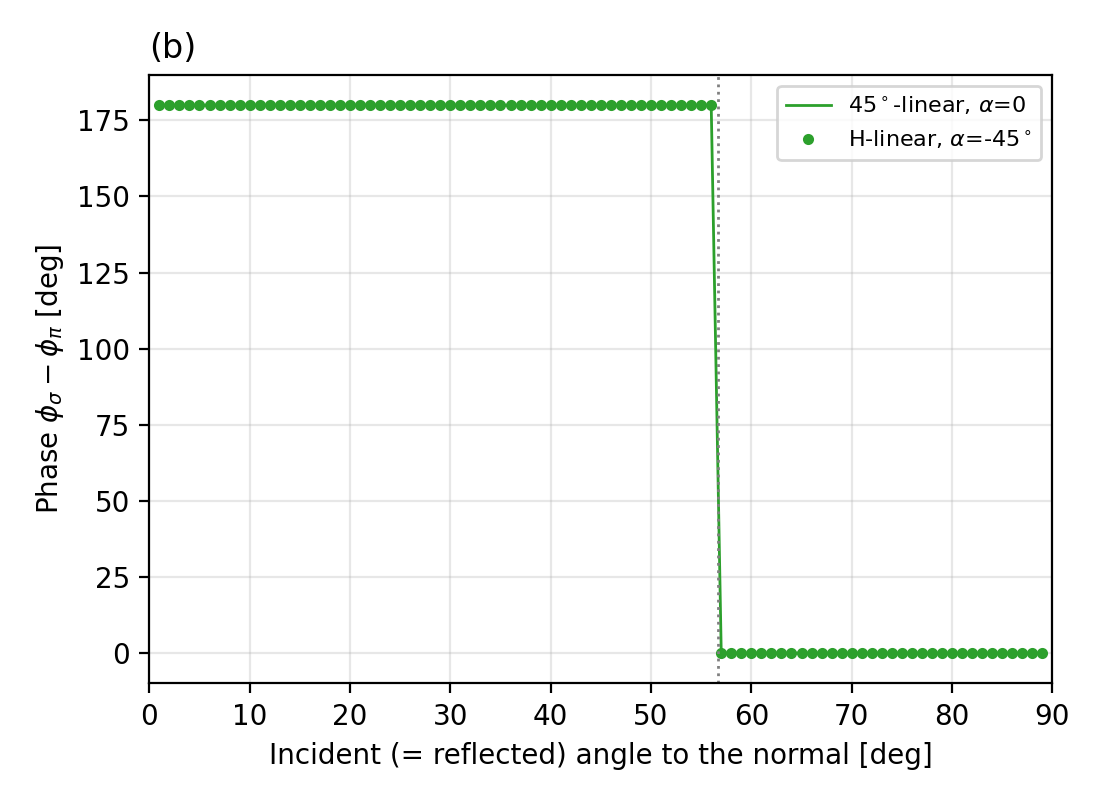
\includegraphics[width=0.95\linewidth]{figures/visiblePhase.png}
\caption{Reflection of a linearly polarized ray by a glass mirror ($n$=1.51), as a function of the incident (or reflected) angle: (a) intensities of the $\sigma$ and $\pi$ components after reflection; (b) change of phase ($\sigma$ minus $\pi$). Lines: beam linearly polarized at 45$^\circ$ and mirror with $\alpha=0$; dots: beam with horizontal linear polarization and mirror with $\alpha=-45^\circ$. The dotted vertical line marks the Brewster angle.}
\label{fig:visible}
\end{figure}

Some examples of exploiting the Brewster angle for applications are:
\begin{itemize}
    \item Photography: Polarizing filters reduce glare by blocking light reflected at the Brewster angle, e.g., from water or glass.
    \item Laser Systems: Brewster windows ensure lasers emit linearly polarized light with minimal reflection.
    \item Polarizing Beam Splitters: Separate s and p polarized light for optical experiments.
    \item Sunglasses: Polarized lenses block glare from horizontal surfaces, strongest at the Brewster angle.
    \item Refractive Index Measurement: Calculate $n=\tan(\theta_{Bw})$ by measuring the Brewster angle.
\end{itemize}

\subsection{X-rays: crystals at $\theta_B\simeq45^\circ$}\label{sec:polarizers45degBenchmark}
We want to study the polarization produced in an x-ray beam by a series of reflections with $\theta_B=\pi/4$. In this case, the crystal reflectivity (in amplitudes) is $r_\sigma \approx 1$ and $r_\pi \approx 0$. The interest of multiple reflections is to eliminate the $\pi$ component by successive reflections (i.e. multiplication) by $r_\pi$.

\subsubsection{Benchmarking}

In this paragraph we consider the Si800 crystal, for which $\theta_B=45^{\circ}$ corresponds to the photon energy 12914.735~eV. There, $\cos(2\theta_B)\approx 0$ and $r_\pi$ practically vanishes. To have a small but non-negligible $\pi$ reflectivity we use the photon energy 12914.0~eV. The Bragg angle at this energy is $\theta_B=45.003257^{\circ}$, and the ``corrected Bragg angle'' (at which the crystal is positioned) is $\theta_{Bc}=45.003592^{\circ}$.
At this corrected Bragg angle, the reflectivities (calculated with {\it crystalpy} for a thick crystal, using {\it xraylib} for the structure factors) are $r_\sigma=-0.0247-0.970 i$ and $r_\pi=(9.33+11.00 i)~10^{-4}$.
The squared modulus, or reflectance, are $R_\sigma=|r_\sigma|^2=0.941660$ and
$R_\pi=|r_\pi|^2=2.081562~10^{-6}$.

Let us use 8 crystals, divided in two packs of 4 crystals each (the ``polariser" and the ``analyser"). A pack has the crystals in non-dispersive configuration $(+,-,+,-)$. The second pack is rotated 90$^\circ$ with respect to the first pack. Therefore we consider all the crystals as a single rigid body, with all crystals well aligned.

We now have to define the incident beam and the orientation of the first crystal with respect to this beam. For our first tests we define an idealized pencil beam (zero cross section, and zero divergence), with a given polarization $P$. In our ray tracing source, all rays are identical. We consider two physically equivalent cases (section~\ref{sec:equivalence}), referred to as case 1 and case 2:
\begin{enumerate}
    \item a source linearly polarized with $P=1$ (Jones vector of each ray $(1,0)^T$) and first crystal rotated -45$^\circ$ along the beam direction (zero is facing up).
    \item a source linearly polarized with $P=0.5$ [Jones vector of each ray $(2^{-1/2},2^{-1/2})^T$] and first crystal is facing up.    
\end{enumerate}

\paragraph{Case 1.}
The Jones vector of the incident ray is $(1,0)^T$ and first crystal is rotated $\alpha$=-45$^\circ$ (therefore $\cos\alpha=2^{-1/2}$ and $\sin\alpha=-2^{-1/2}$). The Jones matrix of the first crystal is:
\begin{equation}\label{eq:Jcase1_xtal1_S4}
    \textbf{J}_1=\textbf{J}_e \cdot \textbf{R}(-45^{\circ})
    =
    2^{-1/2}
    \begin{pmatrix}
r_\sigma  &
-r_\sigma \\
r_\pi&
r_\pi
\end{pmatrix}.
\end{equation}
For the other crystals
\begin{equation}\label{eq:Jcase1_S4}
\textbf{J}_{2,3,4,6,7,8}=
    \begin{pmatrix}
r_\sigma & 0\\
0& 
r_\pi
\end{pmatrix},
\end{equation}
and
\begin{equation}\label{eq:J5case1_S4}
\textbf{J}_{5}=\textbf{J}_e\cdot \textbf{R}(90^{\circ})
=
\begin{pmatrix}
0 & r_\sigma\\
-r_\pi& 0
\end{pmatrix}.
\end{equation}
Strictly, the crystals in the non-dispersive configuration $(+,-)$ are oriented at $\alpha=180^\circ$ with respect to the previous one, so their Jones matrix is $\textbf{J}_e\cdot\textbf{R}(180^\circ)=-\textbf{J}_e$. The six factors $-1$ (crystals 2, 3, 4, 6, 7 and 8) give an overall factor $+1$, and other equivalent choices of the orientation angles (e.g., $270^\circ$ instead of $90^\circ$ for crystal 5) only change the global sign of the final Jones vector, which has no effect on the intensities or on the polarization state. The same applies to case 2.

Therefore, the Jones vector after all reflections is:
\begin{equation}\label{eq:JVcase1_S4}
\left[ \prod_{i=1}^{8} \textbf{J}_i \right]
    \cdot
    \begin{pmatrix}
    1\\0
    \end{pmatrix}=
    2^{-1/2} r_\sigma^4 r_\pi^4
        \begin{pmatrix}
   1&1\\
    -1 & 1
    \end{pmatrix}
    \cdot
        \begin{pmatrix}
    1\\0
    \end{pmatrix}
    =
    2^{-1/2}r_\sigma^4 r_\pi^4
    \begin{pmatrix}
    1\\
    -1
    \end{pmatrix}.
\end{equation}

The intensities (per incident ray of unit intensity) are
\begin{itemize}
    \item $\sigma$-polarized $I_\sigma=|2^{-1/2}~r_\sigma^4 r_\pi^4|^2$=7.38~ 10$^{-24}$
    \item $\pi$-polarized: the same
    \item total 1.48~ 10$^{-23}$.
\end{itemize}
SHADOW4 results are in good agreement (scripts {\tt si800\_rs\_rp\_xraylib.py} and {\tt shadow4\_case\_1\_and\_2.py} in supplementary material).

\paragraph{Case 2.}

The Jones vector of the incident ray is $(2^{-1/2},2^{-1/2})^T$.
The Jones matrices are: 
\begin{equation}\label{eq:Jcase2_S4}
\textbf{J}_{1,2,3,4,6,7,8}=
    \begin{pmatrix}
r_\sigma & 0\\
0& 
r_\pi
\end{pmatrix}
\end{equation}
and
\begin{equation}\label{eq:J5case2_S4}
\textbf{J}_{5}=\textbf{J}_e \cdot \textbf{R}(90^\circ)=
\begin{pmatrix}
0 & r_\sigma\\
-r_\pi& 0
\end{pmatrix}
\end{equation}

Therefore, the Jones vector after all reflections is:
\begin{equation}\label{eq:JVcase2_S4}
\left[ \prod_{i=1}^{8} \textbf{J}_i \right]
    \cdot
    \begin{pmatrix}
    2^{-1/2}\\2^{-1/2}
    \end{pmatrix}=
    r_\sigma^4 r_\pi^4
        \begin{pmatrix}
    0&1\\
    -1 & 0
    \end{pmatrix}
    \cdot
        \begin{pmatrix}
    2^{-1/2}\\2^{-1/2}
    \end{pmatrix}
    =
    2^{-1/2}r_\sigma^4 r_\pi^4
    \begin{pmatrix}
    1\\
    -1
    \end{pmatrix}.
\end{equation}

The intensities are the same as for case 1, and also here SHADOW4 results agree well. 

\subsubsection{A practical case}\label{sec:polarizers45degPractical}

For an X-ray beam within a polarizer utilizing multiple consecutive reflections in channel-cut crystals with a scattering angle of $2\theta_B$=90$^\circ$, despite each reflection yielding a $\pi$-polarization reflectivity of $r_\pi\approx 0$, achieving perfect linear polarization is not feasible for a divergent beam.
Even with an ideal polarizer, the achievable limit for the linear polarization purity $\mathcal{P}$ (ratio of the intensities of the unwanted and wanted linear polarizations) is governed by \cite{Schulze2018}
\begin{equation}\label{eq:polarizer}
    \mathcal{P} = \sigma_h^2 + \sigma_v^2,
\end{equation}
where $\sigma_{h,v}$ are the rms angular divergences in the horizontal and vertical directions of the beam incident on the polarizer.

We simulate the polarimeter used in the experiment of \cite{Schulze2022} at the European XFEL, to verify both the linear purity that can be reached with this setup and the validity of equation~(\ref{eq:polarizer}).
The X-ray source is linearly polarized along the horizontal direction ($P=1$), with rms divergences $\sigma_h$=\SI{273}{\nano\radian} and $\sigma_v$=0, as measured in the experiment.
The photon energy is \SI{6457}{eV} (0.01\% bandwidth), for which the Si 400 reflection has $2\theta_B\approx 90^\circ$.
The polarizer and the analyzer are Si 400 channel-cut crystals, each one with six consecutive reflections in the non-dispersive $(+,-,+,-,+,-)$ configuration, as in \cite{Schulze2022}.
The crystals are calculated as thick crystals with {\it crystalpy} and {\it xraylib}.
$\sigma_h$ is much smaller than the Darwin width of \SI{26}{\micro\radian} of Si 400 at \SI{6457}{eV}.
The scattering plane of the polarizer is vertical, so its $\sigma$ direction is along the electric field of the source. The analyzer is rotated by an angle $\eta$ around the beam with respect to the polarizer, from the parallel ($\eta=0$) to the crossed ($\eta=90^\circ$) setting.
The linear purity achieved by the polarizer and analyzer pair is $\mathcal{P}=I_\text{cross}/I_\text{parallel}$, with $I_\text{parallel}$ and $I_\text{cross}$ the intensities after the analyzer in the parallel and crossed settings, respectively.
The simulations (with $10^5$ rays) are done with the script {\tt shadow4\_practical\_polarizer.py} available in the supplementary material.

Fig.~\ref{fig:polarizer} shows the intensity after the analyzer as a function of $\eta$. It follows $\cos^2\eta$, as for perfect polarizers \cite{Schulze2022}, down to the crossed setting, where $I_\text{parallel}=6704.15$ and $I_\text{cross}=4.85\times 10^{-10}$.
Their ratio gives a linear purity $\mathcal{P}=7.24\times 10^{-14}$, in very good agreement with the value predicted by equation~(\ref{eq:polarizer}), $\mathcal{P}=7.45\times 10^{-14}$, and with the theoretical limit of $7\times 10^{-14}$ given in \cite{Schulze2022} for this source (the measured purity, better than $8\times10^{-11}$, was limited by the background noise). The purity does not depend on the number of reflections of the channel cuts (a polarizer and analyzer with four reflections each give the same result), because it is limited by the divergence of the beam and not by the $\pi$ reflectivity of the crystals.

\begin{figure}
\centering
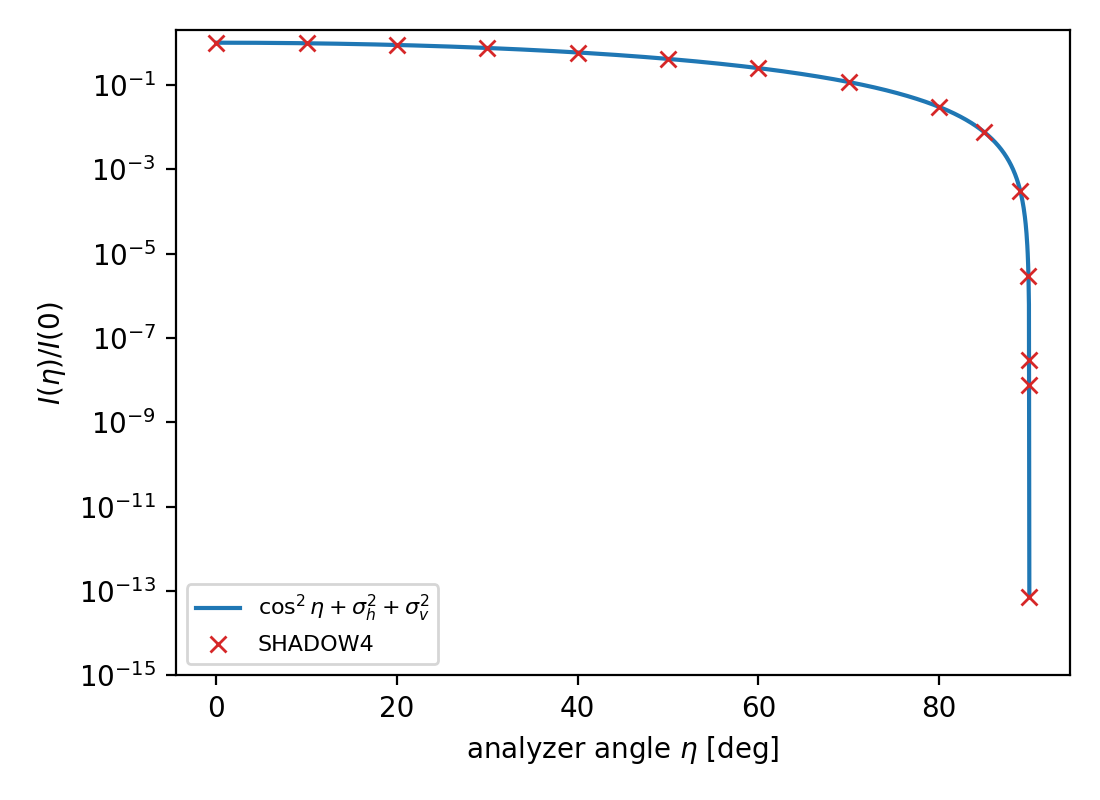
\includegraphics[width=0.85\linewidth]{figures/polarizer.png}
\caption{Simulation of the Si 400 polarimeter at 6457 eV with a source of divergence $\sigma_h$=273 nrad, $\sigma_v$=0: intensity after the analyzer as a function of the analyzer angle $\eta$ ($\eta=0$: parallel, $\eta=90^\circ$: crossed setting), compared with $\cos^2\eta$ plus the limit of equation~(\ref{eq:polarizer}).}
\label{fig:polarizer}
\end{figure}

In the simulation above, the electric vector at the source lies in the horizontal plane, and the polarizer reflects upwards.
For a vacuum birefringence experiment, a linear polarization at 45$^\circ$ is required \cite{Shen2018}, and the polarizer has to be rotated by an angle $\beta=\pm45^\circ$ around the beam, the analyzer being crossed with respect to the polarizer.
The intensity is reduced as $\cos^2\beta$ (a factor 2 for $\beta=\pm45^\circ$), because the projection of the incident electric field on the $\pi$ direction of the polarizer is suppressed.
% The linear purity, however, depends strongly on $\beta$, as shown in Fig.~\ref{fig:polarizer}(b). For the configuration simulated here the results are very well described by
% \begin{equation}\label{eq:polarizerbeta}
%     \mathcal{P}(\beta) = \sigma_h^2\,(1+\sin 2\beta),
% \end{equation}
% which gives $\mathcal{P}\approx 2\sigma_h^2=1.5\times10^{-13}$ for $\beta=45^\circ$ and $\mathcal{P}\approx 0$ for $\beta=-45^\circ$.
% This behaviour can be understood considering that the leakage amplitude of each ray is proportional to a combination $\varphi_\parallel\pm\varphi_\perp$ of its angular deviations parallel and perpendicular to the scattering plane of the polarizer. For divergences that are not correlated in the frame of the polarizer, $\langle(\varphi_\parallel\pm\varphi_\perp)^2\rangle=\sigma_\parallel^2+\sigma_\perp^2$, and equation~(\ref{eq:polarizer}) is recovered. But for a beam with divergence only in the horizontal direction and a polarizer rotated by $\beta$, the two components are correlated ($\varphi_\parallel=\varphi\sin\beta$, $\varphi_\perp=\varphi\cos\beta$), and $\langle(\varphi_\parallel\pm\varphi_\perp)^2\rangle=\sigma_h^2(1\pm\sin 2\beta)$.
% The sign of the asymmetric term depends on the configuration: we found that it changes with the sense of the crossing of the analyzer ($\eta=+90^\circ$ or $-90^\circ$) and with the parity of the number of reflections in the channel cuts.
% Therefore, equation~(\ref{eq:polarizer}) holds when the axes of the beam divergence coincide with the $\sigma$ and $\pi$ directions of the polarizer ($\beta=0$ or $90^\circ$), but, for a beam with asymmetric divergence, a rotated polarizer can give purities between 0 and $2(\sigma_h^2+\sigma_v^2)$, depending on the direction of rotation.

% -----------------------------------------------------------------
% -----------------------------------------------------------------
\section{Phase shifters}\label{sec:phaseshifters_all}
% -----------------------------------------------------------------
% -----------------------------------------------------------------

A phase shifter (or phase retarder) introduces a phase difference between two orthogonal components of the electric field, and converts, e.g., linear into circular polarization. As for the polarizers, we first consider the visible range, with the Fresnel rhomb, and then the X-ray crystal phase plates.

\subsection{Visible range: the Fresnel rhomb}\label{sec:visible_phaseshifters}

As shown in section~\ref{sec:visible_polarizers}, the mirror reflection at Brewster angle is used for obtaining linearly polarized beams when $n_1<n_2$ (e.g. from air to glass with visible light).
To convert linear into circular or elliptical polarization, a phase difference between the $\sigma$ and $\pi$ components is needed. This can be obtained with the total internal reflection, when the beam travels in a denser medium ($n_1>n_2$, e.g. from glass to air) and the incidence angle is larger than the critical angle $\theta_c=\arcsin(n_2/n_1)$. The intensities and the phase change for a single internal reflection glass--air ($n_1=1.51$, $n_2=1$, $\theta_c=41.47^\circ$) calculated with SHADOW4 are shown in Fig.~\ref{fig:internal}. They are obtained in a single run, with a point source emitting 5000 rays at $\lambda=446$~nm, linearly polarized at $45^\circ$ ($P=0.5$, $\Phi=0$), with a uniform vertical divergence of $\pm0.8$~rad around an incidence angle of $45^\circ$, so that the incidence angle covers the interval $0$--$90^\circ$. Below the critical angle the reflection is partial, and the $\pi$ intensity vanishes at the internal Brewster angle $\arctan(n_2/n_1)=33.5^\circ$, where the phase difference jumps from $180^\circ$ to $0$. Above the critical angle the reflection is total for both polarizations, and the phase change $\phi_\sigma-\phi_\pi$ given by equations~(\ref{eq:mirrorphases}) and (\ref{eq:mirrorphasep}) is positive.

\begin{figure}
\centering
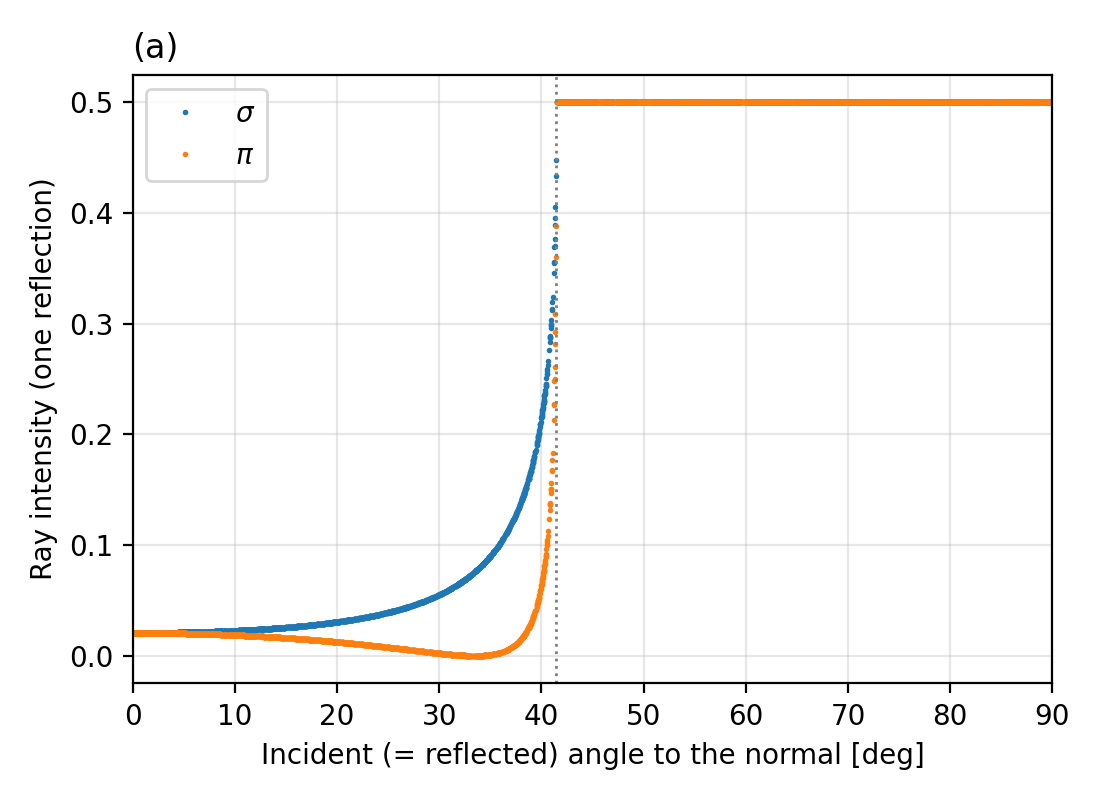
\includegraphics[width=0.95\linewidth]{figures/internalR.png}
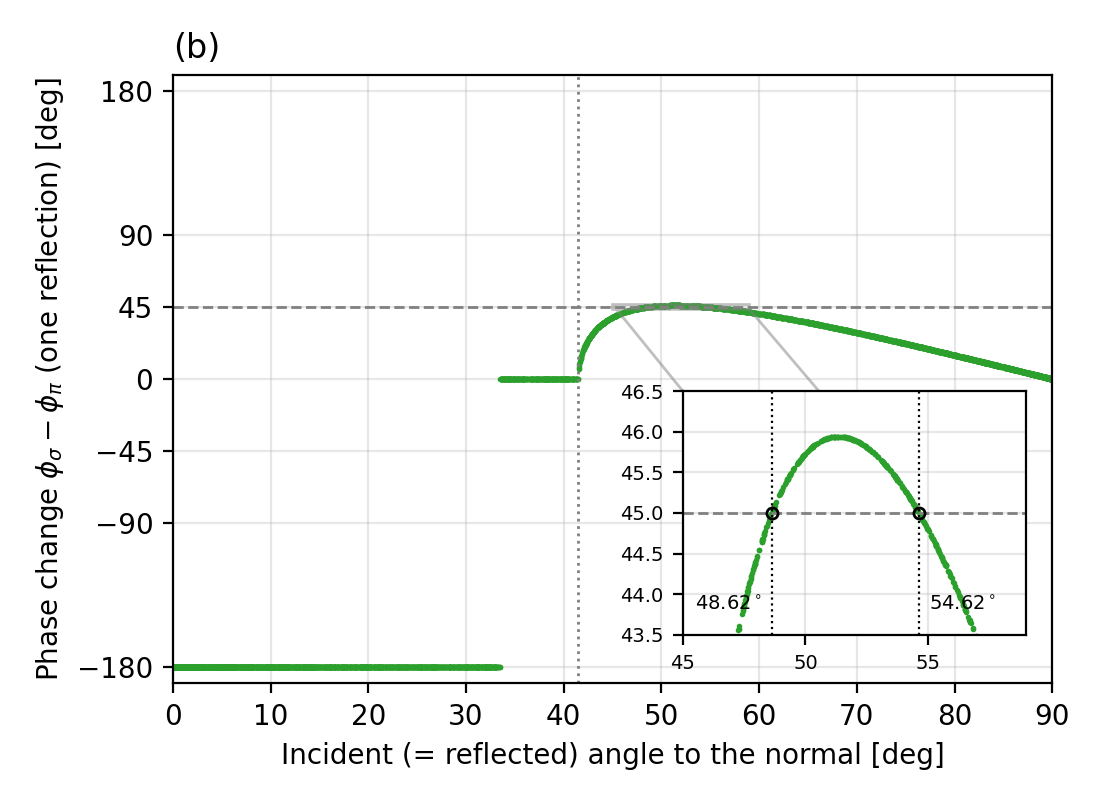
\includegraphics[width=0.95\linewidth]{figures/internalPhase.png}
\caption{Single internal reflection glass--air ($n_1=1.51$, $n_2=1$) of a ray linearly polarized at $45^\circ$, as a function of the incident (or reflected) angle: (a) ray intensity of the $\sigma$ and $\pi$ components (0.5 each for the incident ray); (b) change of phase ($\sigma$ minus $\pi$). The dotted vertical line marks the critical angle, and the dashed horizontal line in (b) the phase change of $45^\circ$. The inset in (b) shows the two incidence angles giving a phase change of $45^\circ$ ($48.62^\circ$ and $54.62^\circ$).}
\label{fig:internal}
\end{figure}

Fig.~\ref{fig:internal}(b) shows an important change of phase in the total reflection zone. To pass from linear polarization (zero phase difference) to circular polarization (phase difference of $90^\circ$), a change of $90^\circ$ is needed, which is not available with a single reflection: the maximum phase change is $45.94^\circ$, at $51.34^\circ$.
But we can use two consecutive reflections adding a phase of $45^\circ$ each, by selecting the appropriate incident angle, as done in the ``Fresnel rhomb" [see Fig.~1.16 in \cite{born_wolf}]. Solving $\phi_\sigma-\phi_\pi=\pi/4$ with equations (\ref{eq:mirrorphases}) and (\ref{eq:mirrorphasep}) gives two solutions, $48.62^\circ$ and $54.62^\circ$ (i.e., $48^\circ37'$ and $54^\circ37'$ as in \cite{born_wolf}).

In the Jones calculus, each total reflection is a phase retarder with a phase difference $\delta=\phi_\sigma-\phi_\pi=\pi/4$, and the Fresnel rhomb is its $N^\text{th}$ power ($N$=2 for two reflections). Applying the rhomb to light linearly polarized at $45^\circ$, with Jones vector $(1,1)^T/\sqrt{2}$ in the SHADOW basis ($P=0.5$, $\Phi=0$, i.e., electric field along $\hat{u}_\sigma+\hat{u}_\pi$; $P_2=-1$ in the standard basis),
\begin{equation}\label{eq:Jrhomb}
\begin{pmatrix}
1  &
0 \\
0&
e^{-i\pi/4}
\end{pmatrix}^2
\frac{1}{\sqrt{2}}\begin{pmatrix}
1  \\
1
\end{pmatrix} = \frac{1}{\sqrt{2}}\begin{pmatrix}
1  \\
-i
\end{pmatrix},
\end{equation}
which, in the standard basis (section~\ref{sec:definitions}), is $(1,i)^T/\sqrt{2}$: left-handed circular polarization, with $P_3=S_3/S_0=+1$.
We checked this with SHADOW4 by ray tracing two internal reflections, with the second surface rotated by $\alpha=180^\circ$ so that the beam exits parallel to the incident one, as in the rhomb. The incidence angle is scanned from $0.1^\circ$ to $89.9^\circ$ (in steps of $0.1^\circ$), tracing for each angle a pencil beam (a single ray) at $\lambda=446$~nm, linearly polarized at $45^\circ$ ($P=0.5$, $\Phi=0$). We evaluate the degree of circular polarization as the ratio $P_3=S_3/S_0$, where $S_3$ is the difference between the intensities of the left-handed and right-handed circularly polarized components and $S_0$ the total intensity. The ray tracing results are shown in Fig.~\ref{fig:rtrhomb}: after the two reflections, $P_3=+1$ (left-handed) at the two solutions above. The same results are obtained in a single run with a point source emitting a fan of rays (uniform vertical divergence of $\pm0.8$~rad around an incidence angle of $45^\circ$), as used for Fig.~\ref{fig:internal}. As expected (section~\ref{sec:equivalence}), the same Stokes parameters, to machine precision, are obtained with a beam with horizontal linear polarization and the rhomb rotated by $\alpha=-45^\circ$ (Fig.~\ref{fig:rtrhomb}), while with $\alpha=+45^\circ$ the light becomes right-handed. This check uses pencil beams, because the vertical fan is not contained in the plane of incidence of the rotated rhomb.

\begin{figure}\label{fig:rtrhomb}
\centering
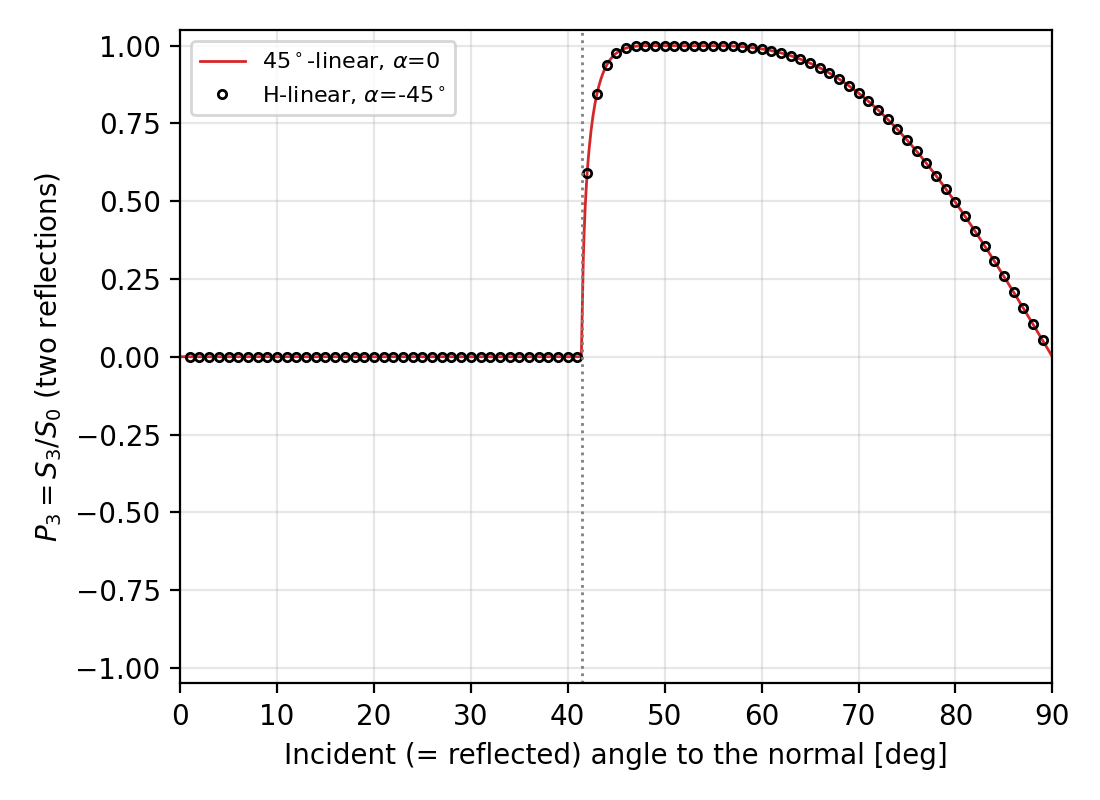
\includegraphics[width=0.95\linewidth]{figures/rtrhomb.png}
\caption{Degree of circular polarization $P_3=S_3/S_0$ after two internal reflections glass--air ($n_1=1.51$, $n_2=1$), as a function of the incident angle. Scans of the incidence angle with pencil beams. Line: incident light linearly polarized at $45^\circ$ and rhomb at $\alpha=0$; circles: horizontal linear polarization and rhomb at $\alpha=-45^\circ$. The Fresnel rhomb is usable over a wide interval of incidence angles: $P_3>0.99$ from $45.9^\circ$ to $59.8^\circ$. The dotted vertical line marks the critical angle.}
\end{figure}

The previous calculations neglect the absorption of the glass. It can be included in the refraction index of the glass, $n_1=1.51+ik$. The relative index of the glass--air interface used by SHADOW4 is then $n_2/n_1=1/(1.51+ik)\simeq1/1.51-ik/1.51^2$, i.e., the equivalent $\beta=-k/n_1^2$ is negative, because the absorbing medium is the incident one. In this case, the root of $n_2\cos\theta_2$ must be chosen with care (Appendix~\ref{sec:mirrorandcrystals}): the outgoing wave for partial reflection and the decaying (evanescent) wave for total reflection. The principal square root, used in previous versions of SHADOW4, gives a growing evanescent wave for total reflection when $\beta<0$, which reverses the phases of $r_\sigma$ and $r_\pi$, and therefore the handedness of the light produced by the rhomb. For the N-BK7 glass at 446~nm, $k=1.08\times10^{-8}$ \cite{RefractiveIndexDatabase2024} and $\beta=-4.7\times10^{-9}$, and the Stokes parameters after the rhomb change by less than $3\times10^{-6}$ at all incidence angles. Even with an absorption $10^5$ times larger ($k=10^{-3}$), $P_3$ changes by less than $2\times10^{-5}$ in the working interval of the rhomb (incidence angles larger than $45^\circ$), and the interval with $P_3>0.99$ is unchanged; the largest changes are found close to the critical angle. Note that, for an absorbing incident medium, the Fresnel equations give a reflectance slightly larger than one in total reflection (for $k=10^{-3}$, the intensity after the two reflections exceeds the incident one by up to 1.8\% for incidence angles larger than $45^\circ$), which is a known consequence of the definition of the reflectance when the incident wave is attenuated, and not a gain. In a real rhomb, the absorption is mainly due to the path of the beam inside the glass (about 0.6\% for 2~cm of N-BK7 at 446~nm), which is the same for the $\sigma$ and $\pi$ components and does not change the polarization; it is not included in the reflection by the SHADOW4 mirror. These calculations are included in the script {\tt shadow4\_fresnel\_rhomb.py}.

Phase shifters in the X-ray range, which use the transmitted beam of perfect crystals, are discussed in the next section.

\subsection{X-rays: crystal phase plates}\label{sec:phasesifters}
X-ray phase plates (phase retarders, or phase shifters) convert the linear polarization of the synchrotron beam into circular or elliptical polarization, and are used routinely at synchrotron beamlines \cite{Freeland2002,Bouchenoire2003,Bouchenoire2012,Francoual2013} and also at free-electron lasers \cite{Suzuki2014}; see \cite{Detlefs2012,Suzuki2023} for the description of the polarization and its control. A widely used phase plate is a thin perfect crystal plate in Bragg geometry, set a few Darwin widths off the Bragg angle, and used in transmission \cite{hirano1993nim,PolarizationDraft}. The transmitted (forward-diffracted) amplitudes $t_\sigma$ and $t_\pi$ (equation~\ref{eq:tbragg}) have similar moduli, but their phase difference $\Delta\phi=\phi_\pi-\phi_\sigma=\arg(t_\pi)-\arg(t_\sigma)$ is large close to the Bragg position, and changes smoothly with the detuning. When the diffraction plane is at $45^\circ$ from the incident linear polarization, the $\sigma$ and $\pi$ components have the same amplitude, and $\Delta\phi=\pm90^\circ$ gives circular polarization (quarter-wave plate).

\subsubsection{Implementation in SHADOW4}

The phase plate is implemented in SHADOW4 in the optical element {\tt S4PlanePhasePlateCrystal} (with its beamline element {\tt S4PlanePhasePlateCrystalElement}), a plane perfect crystal in Bragg geometry with finite thickness $t_c$, for which only the transmitted beam is calculated. For each ray, {\it crystalpy} calculates $t_\sigma$ and $t_\pi$ with equation~(\ref{eq:tbragg}), using the direction and photon energy of the ray, and the Jones matrix $\mathrm{diag}(t_\sigma,t_\pi)$ is applied in the diffraction plane, as explained in section~\ref{sec:forward}. The direction of the ray is not modified (the angle of the outgoing beam is set to $\pi$ minus the incidence angle, both measured from the surface normal), and the ray leaves the crystal from the point where it intercepts the entrance surface (the lateral shift of the ray inside the crystal is neglected).

As for the other crystals, the crystal can be automatically aligned at the Bragg angle (corrected for refraction) for a given photon energy. To this angle, a detuning $\Delta\theta$ can be added (the crystal angle is $\theta_B+\Delta\theta$, $\Delta\theta>0$ meaning a larger glancing angle), either as an angle or in units of the Darwin half width $\omega_s$ for the $\sigma$ polarization, as given by {\it crystalpy}. The orientation of the diffraction plane with respect to the polarization of the incident beam is set with the azimuthal angle $\alpha$ of the crystal (section~\ref{sec:S4}). The element is also available in the OASYS widget ``Phase Plate Crystal''.

\subsubsection{Example: Si 220 phase plate at 10 keV}

We reproduce the Bragg transmission case of \cite{hirano1993nim} (see also \cite{PolarizationDraft}): a Si 220 crystal plate of thickness \SI{50}{\micro\meter} at a photon energy of 10~keV ($\theta_B=18.837^\circ$, $\omega_s=\SI{10.04}{\micro\radian}$). A point source with a uniform vertical divergence of $\pm10\omega_s$ illuminates the crystal, aligned at the Bragg angle without detuning, so that each ray probes a different deviation from the Bragg angle. The intensities of the transmitted rays for the $\sigma$ and $\pi$ polarizations, and the phase difference $\Delta\phi$ between them, are shown in Fig.~\ref{fig:phase_plate}. The results of SHADOW4 coincide with the amplitudes calculated directly with {\it crystalpy} (the maximum differences are $2\times10^{-9}$ in intensity and $3\times10^{-7}$ degrees in phase). Far from the Bragg angle, the transmission is the normal absorption of the plate, $\exp(-\mu t_c/\sin\theta_B)=0.30$. Close to it, the transmission vanishes for the angles of total reflection of the diffracted beam, it is enhanced on the low-angle side (0.35--0.40 at 2--6$\omega_s$, with oscillations reaching $\approx$0.55 near the edge of the reflection), and reduced on the high-angle side (0.14--0.25).

\begin{figure}
\centering
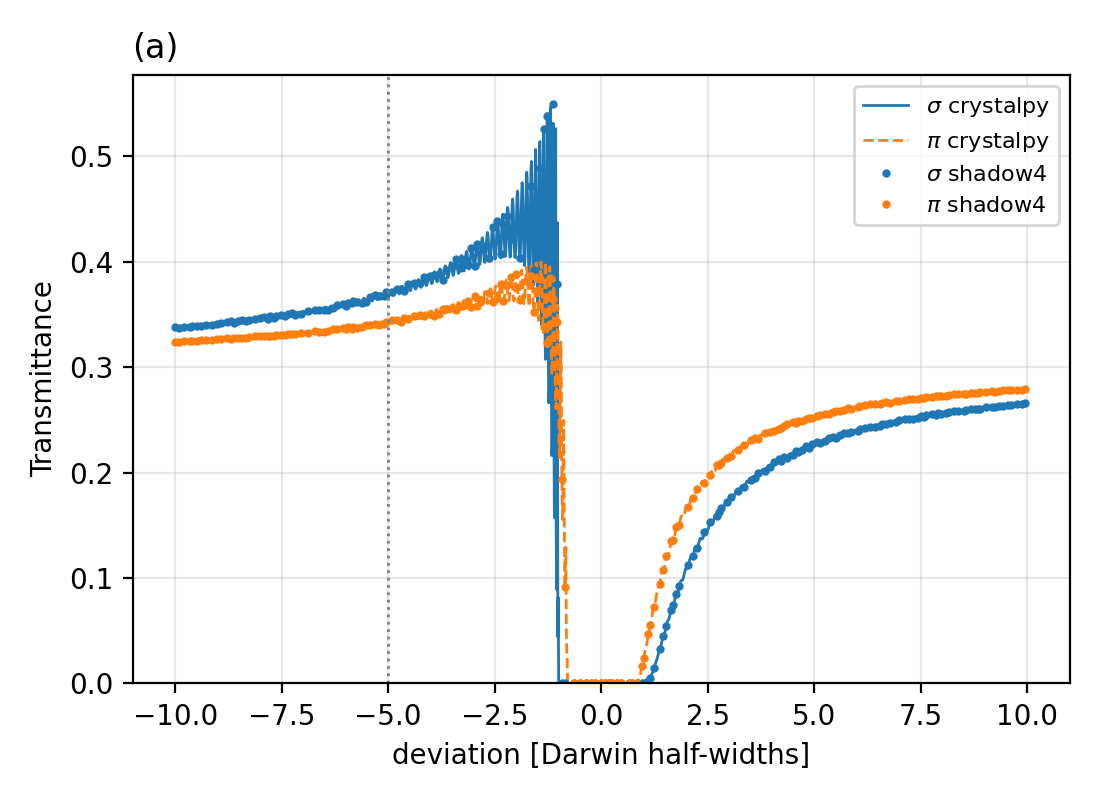
\includegraphics[width=0.95\linewidth]{figures/phase_plate_intensity.png}
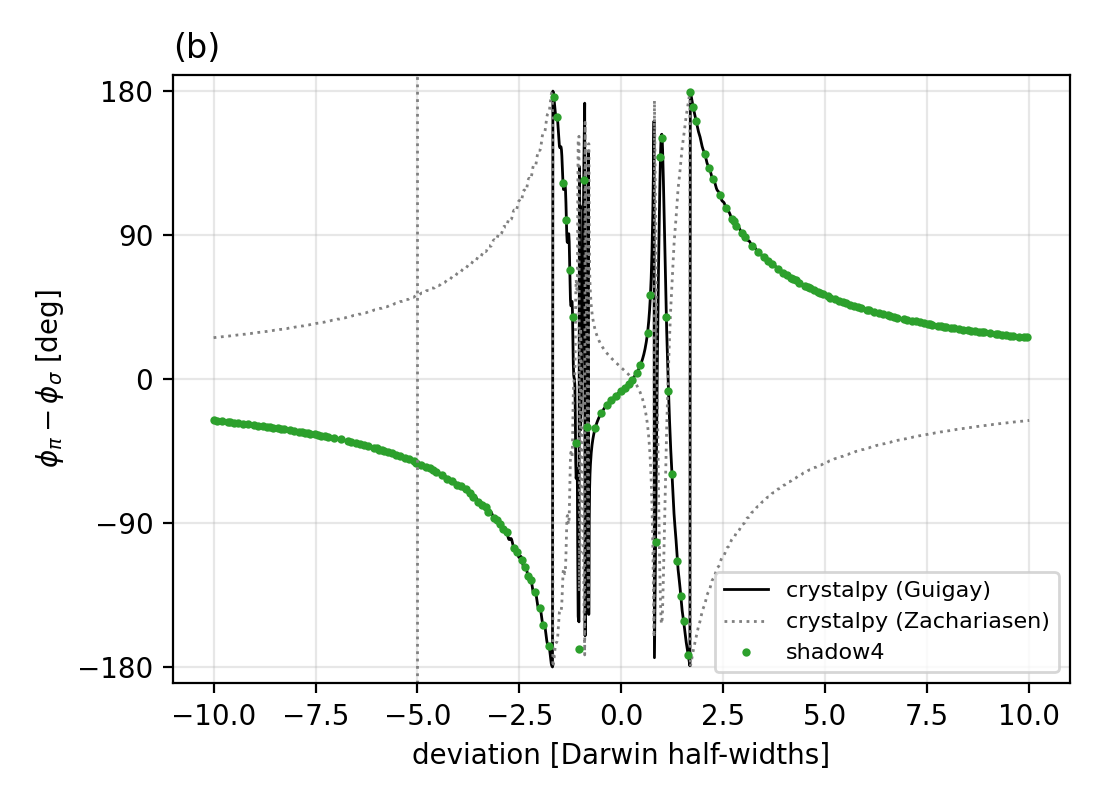
\includegraphics[width=0.95\linewidth]{figures/phase_plate_phase.png}
\caption{Transmitted beam of a Si 220 crystal plate (thickness \SI{50}{\micro\meter}) in Bragg geometry at 10~keV, versus the deviation from the Bragg angle, in units of the Darwin half width $\omega_s$: (a) intensities of the $\sigma$ and $\pi$ components; (b) phase difference $\phi_\pi-\phi_\sigma$. Lines: amplitudes calculated with {\it crystalpy}; dots: SHADOW4 rays (one every ten rays plotted). The dotted gray line in (b) is the result of {\it crystalpy} with the Zachariasen method, which uses the opposite sign convention for the phases (time factor $e^{+i\omega t}$). The vertical dotted line marks the detuning used for the phase plate ($-5\omega_s$).}
\label{fig:phase_plate}
\end{figure}

The phase difference has opposite signs on both sides of the Bragg angle. Its sign depends on the convention for the time factor: with the $e^{-i\omega t}$ convention used in this paper (and in SHADOW4), $\Delta\phi<0$ on the low-angle side, while the curves in \cite{hirano1993nim}, and those obtained with the Zachariasen method in {\it crystalpy}, show the opposite sign (Fig.~\ref{fig:phase_plate}b). A quarter-wave plate ($\Delta\phi=-90^\circ$) is obtained at a detuning of about $-3\omega_s$, with a transmission of 0.38.

The phase plate was then used with a pencil beam with horizontal linear polarization ($P=1$, $\Phi=0$), with the crystal detuned by $-5\omega_s$ (where the transmission is 0.34--0.37, Fig.~\ref{fig:phase_plate}a). For the crystal with $\alpha=0$, the $\sigma$ and $\pi$ intensities of the transmitted ray are $|t_\sigma|^2=0.3666$ and $|t_\pi|^2=0.3433$, and $\Delta\phi=-52.29^\circ$. When the crystal is rotated by $\alpha=\pm45^\circ$ around the beam, the Jones vector of the transmitted ray in the standard basis of the crystal (the $\sigma$ and $\pi$ directions of the diffraction plane) is $(t_\sigma, t_\pi)^T/\sqrt{2}$ for $\alpha=+45^\circ$, and $(t_\sigma, -t_\pi)^T/\sqrt{2}$ for $\alpha=-45^\circ$. The Stokes parameters of the transmitted ray calculated by SHADOW4 are $S_0=0.355$, $P_1=S_1/S_0=0.033$, $P_2=\pm0.611$ and $P_3=\mp0.791$ for $\alpha=\pm45^\circ$, in agreement with these Jones vectors [$P_1=(|t_\sigma|^2-|t_\pi|^2)/(|t_\sigma|^2+|t_\pi|^2)$, $P_2=\pm2|t_\sigma||t_\pi|\cos\Delta\phi/(|t_\sigma|^2+|t_\pi|^2)$, $P_3=\pm2|t_\sigma||t_\pi|\sin\Delta\phi/(|t_\sigma|^2+|t_\pi|^2)$]. Therefore, the transmitted beam has a circular polarization of 79\%, right-handed for $\alpha=+45^\circ$ and left-handed for $\alpha=-45^\circ$ (the two mirror-symmetric configurations of section~\ref{sec:equivalence}). The handedness is also reversed when the detuning changes sign. These results are obtained with the script {\tt shadow4\_phase\_plate.py}.

The SHADOW4 phase plate has also been compared with the polarization of the beam transmitted by a Si 111 phase plate, measured at the P09 beamline of PETRA III (DESY) \cite{Strempfer2013,Francoual2013}. This comparison, which shows the importance of including the angular and energy distributions of the incident beam, is presented in \cite{SanchezdelRio2026desy}.

% -----------------------------------------------------------------
% -----------------------------------------------------------------
\section{Summary and conclusions}
\label{sec:summary}
% -----------------------------------------------------------------
% -----------------------------------------------------------------

We have described how the SHADOW4 ray tracing code represents, transports and modifies the electric field of the rays, and how the polarization of the beam is obtained from it. Each ray carries two electric vectors, along the $\sigma$ and $\pi$ directions, and their phases. SHADOW4 keeps the convention of SHADOW3, in which the triad $(\hat{u}_\sigma,\hat{u}_\pi,\vec{v})$ is left-handed. We have made explicit the relation with the standard (right-handed) formalism of polarization optics: the standard Jones vector is $(\mathcal{E}_\sigma,-\mathcal{E}_\pi)^T$, and the Stokes parameters calculated by SHADOW4, for each ray and for the beam, follow the standard definitions and conventions. They can be used to obtain the polarization ellipse of every ray and of the beam, as shown for a geometrical source and for a bending magnet source.

The interaction of the rays with the optical elements is described with the Jones calculus. For each ray, the incident electric field is projected onto the $\sigma$ and $\pi$ directions of its own scattering plane, multiplied by the complex amplitudes of the element, and expressed along the $\sigma$ and $\pi$ directions of the outgoing ray. This is valid for any orientation of the element with respect to the polarization of the incident beam. The amplitudes are calculated with the Fresnel equations for mirrors, and with the dynamical theory of diffraction ({\it crystalpy}) for perfect crystals, both for the diffracted and the transmitted (forward-diffracted) beams. For the Fresnel equations, the root of $n_2\cos\theta_2$ must correspond to an outgoing or decaying transmitted wave, which is not always the principal root.

The examples show that SHADOW4 reproduces the polarization properties of polarizers and phase shifters in the X-ray and visible ranges:
\begin{itemize}
\item {\it X-ray polarizers.} A polarizer and analyzer made of crystals at $\theta_B\simeq45^\circ$ (Si 800) gives results in agreement with the analytical Jones calculation, for two physically equivalent configurations of the incident polarization and the orientation of the crystals. For the polarimeter used at the European XFEL, the simulated linear polarization purity ($7.24\times10^{-14}$) agrees with the limit imposed by the divergence of the beam ($7.45\times10^{-14}$) and with the theoretical limit given in \cite{Schulze2022} for this setup.
\item {\it Visible polarizers.} The reflection of linearly polarized light by a glass mirror reproduces the Fresnel reflectances and the change of phase at the Brewster angle, and the results do not depend on whether the polarization of the light or the orientation of the mirror is rotated.
\item {\it X-ray phase plates.} A new optical element calculates the transmitted beam of a perfect crystal plate in Bragg geometry, detuned from the Bragg angle. It agrees with direct calculations with {\it crystalpy}, and reproduces the transmission and phase retardation of a Si 220 plate at 10~keV used as phase retarder. A comparison with polarization measurements of a Si 111 phase plate at the P09 beamline of PETRA III is presented in \cite{SanchezdelRio2026desy}.
\item {\it Visible phase shifters.} Two total internal reflections in a Fresnel rhomb convert linear into circular polarization at the incidence angles predicted by the Fresnel equations, with the handedness given by the Jones calculus. The absorption of the glass has a negligible effect on the polarization.
\end{itemize}

The simulations of this paper can be reproduced with the scripts available as supplementary material, and most of them also with the SHADOW4 widgets of the OASYS environment. The electric fields of the rays carry their phases, which are preserved through the beamline; this opens the possibility of using them for the simulation of partially coherent beams, a topic that will be addressed in future work. \todo{check: extension of the Jones treatment to gratings and multilayers}


% %%%%%%%%%%%%%%%%%%%%%%%%%%%%%%%%%%%%%%%%%%%%%%%%
% %%%%%%%%%%%%%%%%%%%%%%%%%%%%%%%%%%%%%%%%%%%%%%%%

\appendix

\section{Reflectivities of mirrors and crystals}\label{sec:mirrorandcrystals}
% -----------------------------------------------------------------
% -----------------------------------------------------------------

\subsection{Mirrors: Fresnel Equations, Brewster Angle, Phases}

Interface between media with refractive indices $n_1$, $n_2$.  
Angles are measured from the \textbf{normal}.

Snell’s law:
\begin{equation}
n_1 \sin\theta_1 = n_2 \sin\theta_2
\end{equation}

\textbf{S-polarization reflection coefficient (amplitude)}
\begin{equation}
r_s =
\frac{n_1 \cos\theta_1 - n_2 \cos\theta_2}
     {n_1 \cos\theta_1 + n_2 \cos\theta_2}
\end{equation}

\textbf{P-polarization reflection coefficient (amplitude)}
\begin{equation}
r_p =
\frac{n_2 \cos\theta_1 - n_1 \cos\theta_2}
     {n_2 \cos\theta_1 + n_1 \cos\theta_2}
\end{equation}

These are the Fresnel equations \cite{born_wolf}. They come from the exact Maxwell boundary-condition solutions. They are valid for X-rays and also for visible light and complex refractive indices.
The sign of $r_p$ corresponds to the SHADOW convention for the $\pi$ versors of the incident and reflected rays [equations~(\ref{eq:u_i}) and (\ref{eq:u_f})]: at grazing incidence ($\theta_1\rightarrow 90^\circ$) $\hat{u}_{\pi,f}\approx\hat{u}_{\pi,i}$ and $r_p\rightarrow r_s\rightarrow -1$, whereas at normal incidence $\hat{u}_{\pi,f}=-\hat{u}_{\pi,i}$ and $r_p=-r_s$, so that the reflected electric vector is the same for any polarization direction, as expected.
For complex refractive indices, $\cos\theta_2=(1-\sin^2\theta_2)^{1/2}$ is a complex number, and the root is chosen so that the transmitted wave in medium 2 (with the time dependence $e^{-i\omega t}$ used in this paper) is outgoing [$\mathrm{Re}(n_2\cos\theta_2)\geq0$] when it propagates, and decaying [$\mathrm{Im}(n_2\cos\theta_2)\geq0$] when it is evanescent (total reflection). For X-rays ($n = 1 - \delta + i\beta$, with $\delta,\beta>0$) this is the root with positive imaginary part of $n_2\cos\theta_2$. The principal square root does not always satisfy these conditions, e.g., for total internal reflection with an absorbing incident medium (section~\ref{sec:visible_phaseshifters}).

The Brewster angle $\theta_{Bw}$ is defined by vanishing p-polarized reflection: $r_p = 0$.
For real refractive indices, from the numerator of $r_p$:
\begin{equation}
\theta_{Bw} = \arctan\left(\frac{n_2}{n_1}\right).
\end{equation}
At the Brewster angle $\theta_{Bw}$:
i) The reflected and refracted rays are perpendicular.
ii) The $p$-polarized reflection vanishes.
iii) Only the $s$-polarization remains reflected.

The phases of $r_s$ and $r_p$ are
obtained from the complex
reflection coefficients:
$r = |r| e^{i\phi}$.

When going from a light to a dense medium ($n_1<n_2$, e.g., air to glass with visible light), the coefficients are real, so $\phi = 0$ or $\phi = \pi$:
\begin{itemize}
\item $r_s < 0 \Rightarrow \phi_s = \pi$
\item $r_p$ changes sign at $\theta_{Bw}$ ($\pi$ phase jump): $r_p>0$ for $\theta_1<\theta_{Bw}$ and $r_p<0$ for $\theta_1>\theta_{Bw}$.
\end{itemize}

For $n_1 > n_2$ (e.g., glass to air with visible light) there is total internal reflection for incidence angles (measured from the normal) larger than the critical angle
\begin{equation}
\theta_c = \arcsin\left(\frac{n_2}{n_1}\right).
\end{equation}
For total internal reflection, $\theta_1 > \theta_c$,
\begin{equation}
|r_s| = |r_p| = 1
\end{equation}
and the phases are (with the time dependence $e^{-i\omega t}$):
\begin{equation}\label{eq:mirrorphases}
\tan\left(\frac{\phi_s}{2}\right)
=
-\frac{\sqrt{\sin^2\theta_1 - (n_2/n_1)^2}}
     {\cos\theta_1},
\end{equation}
\begin{equation}\label{eq:mirrorphasep}
\tan\left(\frac{\phi_p}{2}\right)
=
-\frac{n_1^2}{n_2^2}
\frac{\sqrt{\sin^2\theta_1 - (n_2/n_1)^2}}
     {\cos\theta_1}.
\end{equation}
(The opposite signs are found in references using the time dependence $e^{+i\omega t}$.)
Thus $\phi_s \neq \phi_p$, and the phase difference $\phi_s-\phi_p$ transforms a linear polarization into an elliptical one.

A note on the grazing-incidence approximation for X-rays, used in the Parratt formalism \cite{parratt}. For X-rays,
\begin{equation}
n = 1 - \delta + i\beta,
\end{equation}
with $\delta,\beta \ll 1$. For a small grazing angle $\theta_g=\pi/2-\theta_1$, the normal component of the wavevector in a medium of index $n_j$ is $k_{z,j}=k_0 (n_j^2-\cos^2\theta_g)^{1/2}\approx k_0 f_j$, with
\begin{equation}
f_j = \sqrt{\theta_g^2 - 2\delta_j + 2i\beta_j},
\end{equation}
and the reflection coefficient of the interface between media 1 and 2 is
\begin{equation}
r = \frac{f_1 - f_2}{f_1 + f_2},
\end{equation}
with $f_1=\theta_g$ if medium 1 is vacuum. In this approximation $r_p=r_s$. It is valid for grazing-incidence X-ray reflectivity and multilayers, where it is the basis of Parratt's recursive formalism, but it fails for large angles and does not reproduce the Brewster physics.

Last, we mention that, to make SHADOW4 easier to use for calculations with wavelengths and materials with $n>1$, we implemented tools to retrieve data from the refractive index database \cite{RefractiveIndexDatabase2024} and create SHADOW4 preprocessor files. 

\subsection{Perfect Crystals}

The complex reflection amplitudes of perfect crystals are calculated in SHADOW4 with the {\it crystalpy} library, which implements the solution of the Takagi--Taupin equations for a plane wave incident on an undeformed crystal plate \cite{Guigay2024}. We summarize here the main results, with the notation of \cite{Guigay2024}.

The crystal is characterized by the Fourier components $\chi_0$, $\chi_h$ and $\chi_{-h}$ of the electric susceptibility for the reflection $\mathbf{h}$, written as $u_{0,h,-h}=(k/2)\chi_{0,h,-h}$, with $k=2\pi/\lambda$. The geometry is described by the asymmetry factor $b=\gamma_0/\gamma_h$, with $\gamma_{0,h}$ the direction cosines of the incident and diffracted waves with respect to the inward normal of the crystal surface ($b<0$ for Bragg and $b>0$ for Laue geometry), and by the deviation from the Bragg condition,
\begin{equation}
\Omega = \frac{bh}{2}(\sin\theta - \sin\theta_B) + \frac{b-1}{2}u_0,
\end{equation}
where $h=|\mathbf{h}|$, $\theta$ is the glancing angle of the incident wave on the reflecting planes and $\theta_B$ the Bragg angle ($\Omega$ is denoted $\omega$ in \cite{Guigay2024}). With $a=(bu_hu_{-h}+\Omega^2)^{1/2}$ and $T=t_c/\gamma_0$, where $t_c$ is the crystal thickness, the reflection amplitudes are
\begin{equation}\label{eq:rbragg}
r_{\mathrm{B}} = \frac{-i b u_h \sin(aT)}{a\cos(aT)+i\Omega\sin(aT)}
\end{equation}
for the Bragg case, and
\begin{equation}\label{eq:rlaue}
r_{\mathrm{L}} = i b u_h \frac{\sin(aT)}{a} \exp[iT(u_0+\Omega)]
\end{equation}
for the Laue case. For a thick crystal in Bragg geometry, equation~(\ref{eq:rbragg}) reduces to $r_{\mathrm{B}}^{\mathrm{thick}} = -bu_h/(a+\Omega)$, where the sign of $a$ is chosen such that $|r_{\mathrm{B}}|\rightarrow 0$ far from the Bragg position.

The transmitted (forward-diffracted) amplitudes, i.e., the amplitudes of the wave leaving the crystal along the incident direction, are also obtained from the transfer matrix of the crystal plate \cite{Guigay2024}. They are
\begin{equation}\label{eq:tbragg}
t_{\mathrm{B}} = \frac{a \exp[iT(u_0+\Omega)]}{a\cos(aT)+i\Omega\sin(aT)}
\end{equation}
for the Bragg case, and
\begin{equation}\label{eq:tlaue}
t_{\mathrm{L}} = \left[\cos(aT) - i\frac{\Omega}{a}\sin(aT)\right] \exp[iT(u_0+\Omega)]
\end{equation}
for the Laue case. Far from the Bragg position ($|\Omega|\gg|bu_hu_{-h}|^{1/2}$, so $a\simeq\pm\Omega$), both reduce to $\exp(iTu_0)$, the amplitude of a wave refracted and absorbed along the path $T$ in the crystal, which is the same for the $\sigma$ and $\pi$ polarizations. Close to the Bragg position the transmitted amplitudes $t_\sigma$ and $t_\pi$ differ in modulus and phase, because the diffraction couples the transmitted and diffracted waves with different strengths for both polarizations. This is the basis of the X-ray phase retarders (phase shifters) working in transmission, which use thin crystal plates (typically diamond) in Laue or Bragg geometry, slightly detuned from the Bragg position, where the absorption of the transmitted beam is small and the phase difference $\arg(t_\sigma)-\arg(t_\pi)$ is large \cite{PolarizationDraft}.

These expressions are written for the $\sigma$ polarization. For the $\pi$ polarization, $\chi_h$ and $\chi_{-h}$ are replaced by $C\chi_h$ and $C\chi_{-h}$, with the polarization factor $C=\cos(2\theta_B)$. Note that $C$ is taken with its sign (it is negative for $\theta_B>45^\circ$). This is consistent with the SHADOW definition of the $\pi$ versors, for which $\hat{u}_{\pi,i}\cdot\hat{u}_{\pi,f}=\cos\Theta=\cos(2\theta_B)$ for a symmetric Bragg reflection (section~\ref{sec:S4}). Therefore, the amplitudes $r_\sigma$ and $r_\pi$ calculated by {\it crystalpy} can be directly used as the diagonal elements of the Jones matrix $\textbf{J}_e$ in equation~(\ref{eq:J}). The off-diagonal elements are zero for the charge scattering by a crystal with a scalar susceptibility.

The intensity of the diffracted beam is the reflectance $\mathcal{R}=|r|^2/|b|$, where the factor $1/|b|$ is the ratio of the cross sections of the reflected and incident beams. As SHADOW rays carry intensities, not intensity densities, the elements of the Jones matrix used for the diffracted beams are $r_\sigma/\sqrt{|b|}$ and $r_\pi/\sqrt{|b|}$ (the amplitudes are returned with this factor by {\it crystalpy}). The transmitted beam keeps the cross section of the incident beam, so the transmission amplitudes $t_\sigma$ and $t_\pi$ are used without this factor.


The amplitudes $r_\sigma$ and $r_\pi$ have, in general, different moduli and different phases, which vary across the diffraction profile. This difference is the basis of the crystal polarization optics: at $\theta_B=45^\circ$ we have $C=0$ and $r_\pi=0$, so the crystal is a linear polarizer (section~\ref{sec:polarizers45degBenchmark}), and the phase difference between $t_\sigma$ and $t_\pi$ (and also between $r_\sigma$ and $r_\pi$) in the tails of the diffraction profile is used in crystal phase retarders \cite{PolarizationDraft}.

In the ray tracing, the amplitudes are calculated for each ray, with its own incidence direction and photon energy, and the local normal to the crystal surface at the intercept point. For curved crystals this assumes that the local reflectivity is that of a flat crystal \cite{Guigay2024}. The direction of the diffracted ray is $\mathbf{k}_{out}=\mathbf{k}_h+\beta\mathbf{n}$, with $\mathbf{k}_h=\mathbf{k}_0+\mathbf{h}$, $\mathbf{n}$ the unit vector along the inward normal to the crystal exit surface, and $\beta$ obtained from the condition $|\mathbf{k}_{out}|=k$ \cite{Guigay2024}.

% -----------------------------------------------------------------
% -----------------------------------------------------------------
\section{Interaction with the beamline element in SHADOW3}\label{sec:S3}
% -----------------------------------------------------------------
% -----------------------------------------------------------------

SHADOW3 did not use the Jones calculus. The electric vectors of the incident ray were projected onto the local $\sigma$ and $\pi$ directions, multiplied by the reflectivities and phases of the element, and then modified to restore their orthogonality to the outgoing direction. This procedure, described here for reference, is not equivalent to the Jones calculus of section~\ref{sec:S4} when the element is rotated with respect to the polarization of the incident ray.

The effect of the beamline element (reflection/refraction/diffraction) is applied to the beam. In SHADOW3, once the beam arrives to the element, the changes are done in three steps 
\begin{enumerate}
    \item change the incoming electric vectors to the local $\sigma$ and $\pi$ directions.
    \item multiplication of the electric fields by the reflectivities $R_\sigma$ and $R_\pi$ and change the phases accordingly.
    \item modify the outcoming electric field to guarantee the orthogonality with the output (reflected/refracted/diffracted) direction.
\end{enumerate}

% -----------------------------------------------------------------
\subsection{Modifications of electric fields in ``local'' o.e.}
\label{sec:localoe}
% -----------------------------------------------------------------
% -----------------------------------------------------------------


The physics of the X-ray reflection and diffraction in an optical surface affects in a different way 
the {\it local} parallel ($\sigma$) and perpendicular ($\pi$) components. The ``local'' parallel component
is a vector that sits on the o.e. surface and it is not coincident with the incident $\vec{E}_\sigma$.
Therefore, one must calculate the ``local'' $\vec{u}'_\sigma$ and $\vec{u}'_\pi$ vectors that verify
1) they are orthogonal to $\vec{v}$ and ii) $\vec{u}'_\sigma$ is contained in the o.e. surface. 
This is done in the method {\tt get\_local\_directions\_sigma\_pi} of {\tt S4Beam}.

% \begin{lstlisting}[caption={Method of {\tt S4Beam} to compute the local directions $\sigma$ and $\pi$ at the beamline element.}, label={lst:localsigmaandpi}, captionpos=b]
%     def get_local_directions_sigma_pi(self, vNormal, vIn=None):
%         """
%         Given a direction N (normal to a surface), this routine calculates the "local sigma and pi"
%         directions, or the unitary vectors perpendicular and parallel to the scattering plane, respectively.
%         The scattering plane is defines as the plane that contains N and the ray direction vIn.

%         Parameters
%         ----------
%         vNormal: numpy array
%             An array of vectors (npoints, 3) with the normal N.
%         vIn: numpy array, optional
%             The array of vectors with the incident direction. If None, it uses the direction in the S4Beam.

%         Returns
%         -------
%             tuple:
%             (direction_sigma, direction_pi) the two unitary array of vectors with the sigma and pi-directions.
%         """
%         if vNormal.shape[1] != 3:
%             raise Exception("vNormal must be an array of vectors (npoints, 3).")

%         if vIn is None: vIn = self.get_columns([4, 5, 6]).T

%         E_S = self.get_columns([7, 8, 9]).T
%         E_P = self.get_columns([16, 17, 18]).T

%         # ! * ... we have to compute
%         # ! * some angles, namely the sine of the incidence angle and the sine
%         # ! * of the A vector with the normal. Also, the polarized light is
%         # ! * treated as a superposition of two orthogonal A vectors with the appropriate
%         # ! * phase relation. These two incoming vectors have to be resolved into the
%         # ! * local S- and P- component with a new phase relation.
%         # ! * A_VEC will be rotated later, once the amplitude will have been determined.
%         #      	CALL	CROSS 	(VVIN,VNOR,AS_TEMP)	! vector pp. to inc.pl.
%         #      	IF (M_FLAG.EQ.1) THEN
%         # 	        CALL	DOT	(AS_VEC,AS_VEC,AS2)
%         # 	        CALL	DOT	(AP_VEC,AP_VEC,AP2)
%         # 	        IF (AS2.NE.0)	THEN
%         #              	 DO 499 I=1,3
%         #  499   	            AS_TEMP(I) = AS_VEC(I)
%         # 	        ELSE
%         # 	             DO 599 I=1,3
%         #  599	            AS_TEMP(I) = AP_VEC(I)
%         # 	        END IF
%         #      	END IF
%         #      	CALL	NORM  	(AS_TEMP,AS_TEMP)	! Local unit As vector
%         # CALL	CROSS	(AS_TEMP,VVIN,AP_TEMP)
%         # CALL	NORM	(AP_TEMP,AP_TEMP)	! Local unit Ap vector

%         v_S = vector_cross(vIn, vNormal)  # AS_TEMP
%         v_Smod = vector_modulus(v_S)
%         mask = (v_Smod == 0.0)
%         if mask.any():
%             print(">>>>>>>>>> FOUND A ZERO!!!!!")
%             if v_Smod.sum() > 0:
%                 v_S[mask, 0] = E_S[mask, 0]
%                 v_S[mask, 1] = E_S[mask, 1]
%                 v_S[mask, 2] = E_S[mask, 2]
%             else:
%                 v_S[mask, 0] = E_P[mask, 0]
%                 v_S[mask, 1] = E_P[mask, 1]
%                 v_S[mask, 2] = E_P[mask, 2]

%         v_P = vector_cross(v_S, vIn)
%         uS = vector_norm(v_S)
%         uP = vector_norm(v_P)

%         return vector_norm(v_S), vector_norm(v_P)
% \end{lstlisting}


The electric vector can thus be expressed in two orthonormal vectors $\vec{E'}_\sigma$ and $\vec{E'}_\pi$ along these 
new directions $\vec{u'}_\sigma$ and $\vec{u'}_\pi$. Physically, it is a rotation of the old electric vectors around
the $\vec{v}$ direction to put the $\sigma$ component on top of the surface, but the rotation affect not only the 
moduli, but also the phases. The new (complex) electric vectors are build from the projection of the old ones onto the
new axes, thus originating a transformation in both moduli and phases:

\begin{eqnarray}
\vec{E'}_\sigma e^{i \phi'_\sigma} = [(\vec{E}_\sigma e^{i \phi_\sigma}).\vec{u'}_\sigma + (\vec{E}_\pi e^{i \phi_\pi}).\vec{u'}_\sigma ] 
  ~~\vec{u'}_\sigma  \\ 
\vec{E'}_\pi e^{i \phi'_\pi} = [(\vec{E}_\sigma e^{i \phi_\sigma}).\vec{u'}_\pi + (\vec{E}_\pi e^{i \phi_\pi}).\vec{u'}_\pi ] 
  ~~\vec{u'}_\pi 
\end{eqnarray}


Defining the projection of the (real) electric field components onto these versors as: 
\begin{eqnarray}
a_{11} = \vec{E}_\sigma . \vec{u'}_\sigma, ~~~~ 
a_{12} = \vec{E}_\inred{\pi} . \vec{u'}_\inred{\sigma} \nonumber \\
a_{21} = \vec{E}_\inred{\sigma} . \vec{u'}_\inred{\pi}, ~~~~
a_{22} = \vec{E}_\pi . \vec{u'}_\pi 
\end{eqnarray}

we get:
\begin{eqnarray}
\label{withphases}
\vec{E'}_\sigma e^{i \phi'_\sigma} = (a_{11} e^{i \phi_\sigma} + a_{12} e^{i \phi_\pi}) \vec{u'}_\sigma \nonumber \\ 
\vec{E'}_\pi e^{i \phi'_\pi} =    (a_{21} e^{i \phi_\sigma} + a_{22} e^{i \phi_\pi}) \vec{u'}_\pi
\end{eqnarray}

And the moduli are: 

\begin{eqnarray}
|\vec{E'}_\sigma|^2 = \vec{E'}_\sigma . \vec{E'}_\sigma^*  = 
a_{11}^2 + a_{12}^2 + 2 a_{11} a_{12} \cos(\phi_\sigma-\phi_\pi) \equiv
M_\sigma^2 \nonumber \\ 
|\vec{E'}_\pi|^2    = \vec{E'}_\pi    . \vec{E'}_\pi^*     = 
a_{21}^2 + a_{22}^2 + 2 a_{21} a_{22} \cos(\phi_\sigma-\phi_\pi) \equiv
M_\pi^2
\end{eqnarray}

Therefore we can construct the new local (real) electric fields as: 
\begin{eqnarray}
\label{final1}
\vec{E'}_\sigma = M_\sigma \vec{u'}_\sigma  \nonumber \\ 
\vec{E'}_\pi = M_\pi \vec{u'}_\pi  
\end{eqnarray}

To compute the new phases, we insert Eq.~\ref{final1} in Eq.~\ref{withphases} and get: 
\begin{eqnarray}
e^{i \phi'_\sigma} = M_\sigma^{-1} (a_{11} e^{i \phi_\sigma} + a_{12} e^{i \phi_\pi})  \nonumber \\ 
e^{i \phi'_\pi} =  M_\pi^{-1}      (a_{21} e^{i \phi_\sigma} + a_{22} e^{i \phi_\pi}) 
\end{eqnarray}

Therefore:
\begin{eqnarray}
\label{final2}
\tan{\phi'_\sigma} = \frac{Im(a_{11} e^{i \phi_\sigma} + a_{12} e^{i \phi_\pi})}
                          {Re(a_{11} e^{i \phi_\sigma} + a_{12} e^{i \phi_\pi})} = 
                          \frac{a_{11} \sin{\phi_\sigma} + a_{12} \sin{\phi_\pi}}
                               {a_{11} \cos{\phi_\sigma} + a_{12} \cos{\phi_\pi}}  \nonumber \\ 
\tan{\phi'_\pi} =  \frac{Im(a_{21} e^{i \phi_\sigma} + a_{22} e^{i \phi_\pi})}
                        {Re(a_{21} e^{i \phi_\sigma} + a_{22} e^{i \phi_\pi})} = 
                        \frac{a_{21} \sin{\phi_\sigma} + a_{22} \sin{\phi_\pi}}
                             {a_{21} \cos{\phi_\sigma} + a_{22} \cos{\phi_\pi}}
\end{eqnarray}


These equations were implemented in SHADOW3.

% \begin{lstlisting}[caption={Code to compute the local $\sigma$ and $\pi$ electric fields at the beamline element.}, label={lst:rotationelements}, captionpos=b]
%             #
%             # STEP 1: get local sigma and pi directions v_S and v_P (uS and uP unitary vectors)
%             #

%             uS, uP = footprint.get_local_directions_sigma_pi(vH, vIn=vIn)

%             #
%             # calculate the electric field in the local coordinate system
%             #

%             # CALL	DOT	(AS_VEC,AS_TEMP,A11)	! matrix element of rotation
%             # CALL	DOT	(AP_VEC,AS_TEMP,A12)	! matrix element of rotation
%             # CALL	DOT	(AS_VEC,AP_TEMP,A21)	! matrix element of rotation
%             # CALL	DOT	(AP_VEC,AP_TEMP,A22)	! matrix element of rotation
%             # ! ** Now recompute the ampltitude and phase of the local S- and P- component.
%             # AS_NEW	= SQRT(ABS(A11**2 + A12**2 +  &
%             #         2.0D0*A11*A12*COS(PHS-PHP)))
%             # AP_NEW	= SQRT(ABS(A21**2 + A22**2 +  &
%             #         2.0D0*A21*A22*COS(PHS-PHP)))
%             # CALL	SCALAR	(AS_TEMP,AS_NEW,AS_VEC)	! Local As vector
%             # CALL	SCALAR	(AP_TEMP,AP_NEW,AP_VEC)	! Local Ap vector
%             # PHTS	= A11*SIN(PHS) + A12*SIN(PHP)
%             # PHBS	= A11*COS(PHS) + A12*COS(PHP)
%             # PHTP	= A21*SIN(PHS) + A22*SIN(PHP)
%             # PHBP	= A21*COS(PHS) + A22*COS(PHP)
%             # CALL	ATAN_2	(PHTS,PHBS,PHS)		! Phase of local As vector
%             # CALL	ATAN_2	(PHTP,PHBP,PHP)		! Phase of local Ap vector
%             # ! C
%             # ! C
%             # CALL	DOT	(VVIN,VNOR,SIN_VAL)	! sin(graz. ang)
%             # CALL	DOT	(Q_OUT,VNOR,SIN_REF)	! sin(graz.ref.ang)

%             a11 = vector_dot(E_S, uS)
%             a12 = vector_dot(E_P, uS)
%             a21 = vector_dot(E_S, uP)
%             a22 = vector_dot(E_P, uP)

%             M2_S = a11 ** 2 + a12 ** 2 + 2 * a11 * a12 * numpy.cos(PhiS - PhiP)
%             M2_P = a21 ** 2 + a22 ** 2 + 2 * a21 * a22 * numpy.cos(PhiS - PhiP)

%             E_local_S = vector_multiply_scalar(uS, numpy.sqrt(M2_S))
%             E_local_P = vector_multiply_scalar(uP, numpy.sqrt(M2_P))

%             local_PhiS = numpy.arctan2((a11 * numpy.sin(PhiS) + a12 * numpy.sin(PhiP)) , (a11 * numpy.cos(PhiS) + a12 * numpy.cos(PhiP)))
%             local_PhiP = numpy.arctan2((a21 * numpy.sin(PhiS) + a22 * numpy.sin(PhiP)) , (a21 * numpy.cos(PhiS) + a22 * numpy.cos(PhiP)))
%             # END OF STEP 1
% \end{lstlisting}


Note that these transformations imply a polarization mixing, or not conservation of the intensity of each component during the projection ($|\vec{E'}_\sigma| \ne |\vec{E}_\sigma|$),
but the total intensity is conserved ($I=|\vec{E}_\sigma|^2+|\vec{E}_\pi|^2=
|\vec{E'}_\sigma|^2+|\vec{E'}_\pi|^2$). The phases also change.
% but the difference of thase is conserved $\Phi=\phi_\sigma-\pi_\pi=\phi'_\sigma-\phi'_\pi$ (I think, but I have not demostrated it).
The new electric vectors are orthogonal to $\vec{v}$ by constructions.

% -----------------------------------------------------------------
\subsection{Reflection/refraction in the o.e. and subsequent changes in electric vectors}
\label{sec:reflection}
% -----------------------------------------------------------------

Once the electric vectors are expressed in the o.e. local coordinates ($\vec{E'}_\sigma$ and 
$\vec{E'}_\pi$) they are multiplied by the mirror/crystal reflectivities and the phases also affected: : 
\begin{eqnarray}
 \label{reflectivities}
 \vec{E'}_\sigma^{new} = \vec{E'}_\sigma R_\sigma, \nonumber \\
 \vec{E'}_\pi^{new} = \vec{E'}_\pi R_\pi, \nonumber \\
 {\phi '}_\sigma^{new} = {\phi '}_\sigma + \Sigma_\sigma, \nonumber \\
 {\phi '}_\pi^{new} = {\phi '}_\pi + \Sigma_\pi,
\end{eqnarray}
where $R_\sigma$ and $R_\pi$ are the o.e. reflectivities and $\Sigma_\sigma$ and $\Sigma_\pi$ are the  phases added in the reflection/refraction/diffraction. 

% -----------------------------------------------------------------
\subsection{subsequent changes in electric vectors to guarantee orthogonality}
\label{sec:orthogonality}
% -----------------------------------------------------------------

The resulting electric vectors and phases after applying Eq.~\ref{reflectivities} must now hold the orthogonality relations (Eq.~\ref{ortho}) with respect to the new direction $\vec{v'}$, therefore they must be changed. 

% \color{red}
% This part was incorrectly
% done in the following code, which assumes conservation of the $\vec{E'}_\sigma$ component (except for gratings)
% and the $\pi$ component is ``mirrored''. These operations do not garantee that the resulting 
% vectors are normal to $\vec{v'}$. In some cases, in particular for $\sigma$ polarizad light onto 
% o.e.'s with mirror orientation angle $90^\circ$ can result in a loss of beam intensity in 
% subsequent changes of frames. The {\bf wrong} code was (in {\tt MIRROR1}): 
% \color{black}

% \begin{lstlisting}
% ! ** So far we have the new amplitude of the two components. We have now
% ! ** to 'reflect' A_VEC onto the mirror. For this, notice that the s-comp
% ! ** is geometrically unchanged, while the p-comp is changed. The angles
% ! ** are exchanged with respect to VVIN. Things are more complicated in
% ! ** the case of a grating, due to the vectorial nature of the diffraction,
% ! ** not treated here. We make the simplifying assumption that the
% ! ** diffraction will not change the degree of polarization. This mean that
% ! ** A_VEC will have the same components referred to the ray as before the
% ! ** diffraction. 

% VVOUT(1)	=   RAY(4,ITIK)
% VVOUT(2)	=   RAY(5,ITIK)
% VVOUT(3)	=   RAY(6,ITIK)
% ! C 
% ! C The following IF block applies only to the GRATING case.
% ! C The binormal is redefined in terms of the diffraction
% ! C plane.
% ! C
%      	IF (F_GRATING.NE.0.OR.F_BRAGG_A.EQ.1) THEN
% 	  CALL	PROJ	(VVOUT,VNOR,VTEMP)
% 	  CALL	SCALAR	(VTEMP,-2.0D0,VTEMP)
% 	  CALL	SUM	(VTEMP,VVOUT,VTEMP)
% 	  !CALL	CROSS	(VTEMP,VNOR,AS_TEMP)
% 	  CALL	CROSS_M_FLAG	(VTEMP,VNOR,AS_TEMP,M_FLAG)
%      	 IF (M_FLAG.EQ.1) THEN
% 	   CALL	DOT	(AS_VEC,AS_VEC,AS2)
% 	   CALL	DOT	(AP_VEC,AP_VEC,AP2)
% 	  IF (AS2.NE.0)	THEN
%      	    DO 899 I=1,3
%  899          AS_TEMP(I) = AS_VEC(I)
% 	  ELSE
% 	   DO 999 I=1,3
%  999	     AS_TEMP(I) = AP_TEMP(I)
%      	  END IF
% 	 END IF
%      	  CALL	NORM  	(AS_TEMP,AS_TEMP)	! Local unit As vector
% 	  CALL	CROSS	(AS_TEMP,VTEMP,AP_TEMP)
% 	  CALL	NORM	(AP_TEMP,AP_TEMP)	! Local unit Ap vector
%      	  CALL	DOT	(AS_VEC,AS_VEC,RES)
%      	  RES	=    SQRT (RES)

%      	  CALL	SCALAR	(AS_TEMP,RES,AS_VEC)
% 	  CALL	DOT	(AP_VEC,AP_VEC,RES)
% 	  RES	=    SQRT (RES)
% 	  CALL	SCALAR	(AP_TEMP,RES,AP_VEC)
%      	END IF


% CALL	PROJ	(AP_VEC,VNOR,VTEMP)
% CALL	VECTOR	(VTEMP,AP_VEC,VTEMP)
% CALL	SCALAR	(VTEMP,-2.0D0,VTEMP)

% CALL	SUM	(AP_VEC,VTEMP,AP_VEC)
% \end{lstlisting}

% \color{red}

The code simply calculates the new $\sigma$ and $\pi$ versors orthogonal to $\vec{v'}$ and affects them by the electric field moduli that do not change. 
Also, the phases are not changed. 
This guarantees that the intensity is conserved, as well as orthogonality.


% \color{black}

% \begin{lstlisting}[caption={\todo{CORRECT!!} Code to guarantee that the local $\sigma$ and $\pi$ electric fields hold the orthogonality relationships.}, label={lst:finalorthogonality}, captionpos=b]
%             #
%             # STEP 3
%             #

%             # ! Electric vectors are changed to assure orthogonality with the new direction VVOUT
%             # ! To conserve intensity, the moduli of Es and Ep must not change
%             # ! AS_VEC and VVOUT are not orthogonal so a projection of S and P coordinates into the
%             # ! new ones do not work as it may be a component of the electric field along VVOUT
%             #
%             # CALL CROSS_M_FLAG  (VVOUT,VNOR,AS_TEMP,M_FLAG) ! vector pp. to inc.pl.
%             # CALL DOT (AS_VEC,AS_VEC,AS2)
%             # CALL DOT (AP_VEC,AP_VEC,AP2)
%             #
%             # IF (M_FLAG.EQ.1) THEN
%             #  IF (AS2.NE.0) THEN
%             #    DO I=1,3
%             #      AS_TEMP(I) = AS_VEC(I)
%             #    END DO
%             #  ELSE
%             #   DO I=1,3
%             #    AS_TEMP(I) = AP_VEC(I)
%             #   END DO
%             #  END IF
%             # END IF
%             #
%             # CALL NORM   (AS_TEMP,AS_TEMP) ! Local unit As vector perp to vvout
%             # CALL CROSS (AS_TEMP,VVOUT,AP_TEMP)
%             # CALL NORM (AP_TEMP,AP_TEMP) ! Local unit Ap vector perp to vvout
%             #
%             # do i=1,3
%             #   as_vec(i) = as_temp(i) * sqrt(as2)
%             #   ap_vec(i) = ap_temp(i) * sqrt(ap2)
%             # end do

%             aS = vector_modulus(E_diffracted_S)
%             aP = vector_modulus(E_diffracted_P)

%             v_S = vector_cross(vOut, vH) # AS_TEMP
%             v_Smod = vector_modulus(v_S)
%             mask = (v_Smod == 0.0)
%             if mask.any():
%                 print(">>>>>>>>>> FOUND A ZERO!!!!!")
%                 if v_Smod.sum() > 0:
%                     v_S[mask, 0] = E_diffracted_S[mask, 0]
%                     v_S[mask, 1] = E_diffracted_S[mask, 1]
%                     v_S[mask, 2] = E_diffracted_S[mask, 2]
%                 else:
%                     v_S[mask, 0] = E_diffracted_P[mask, 0]
%                     v_S[mask, 1] = E_diffracted_P[mask, 1]
%                     v_S[mask, 2] = E_diffracted_P[mask, 2]

%             v_P = vector_cross(v_S, vOut) # AP_TEMP

%             uS = vector_norm(v_S)
%             uP = vector_norm(v_P)

%             E_diffracted_S[:, 0] = uS[:, 0] * aS
%             E_diffracted_S[:, 1] = uS[:, 1] * aS
%             E_diffracted_S[:, 2] = uS[:, 2] * aS

%             E_diffracted_P[:, 0] = uP[:, 0] * aP
%             E_diffracted_P[:, 1] = uP[:, 1] * aP
%             E_diffracted_P[:, 2] = uP[:, 2] * aP

%             # END STEP 3
% \end{lstlisting}

%%%%%%%%%%%%%%%%%%%%%%

\newpage

% -----------------------------------------------------------------
\section{Scripts}\label{sec:scripts}
% -----------------------------------------------------------------

The Python scripts used for the examples are available as supplementary material (Table~\ref{tab:scripts}). They use SHADOW4 and, for some calculations, {\it crystalpy} and {\it xraylib}.

\begin{table}
\caption{Scripts used for the examples of this paper.}
\label{tab:scripts}
\begin{tabular}{p{0.45\linewidth}p{0.47\linewidth}}
\hline
Script & Example \\
\hline
{\tt stokes\_geometrical\_source.py} & Jones vectors and Stokes parameters of the geometrical source (Table~\ref{tab:source_polarization}) \\
{\tt shadow4\_polarization\_ellipse.py} & Polarization ellipses (Figs.~\ref{fig:ellipse_geometrical} and \ref{fig:ellipse_bm}) \\
{\tt shadow4\_insertion\_devices\_stokes.py} & Stokes parameters of a bending magnet versus $Z'$ (Fig.~\ref{fig:bm_stokes}) \\
{\tt shadow4\_visible\_polarizer3.py} & Glass mirror at the Brewster angle (Fig.~\ref{fig:visible}) \\
{\tt si800\_rs\_rp\_xraylib.py}, {\tt shadow4\_case\_1\_and\_2.py} & Si 800 polarizer and analyzer (section~\ref{sec:polarizers45degBenchmark}) \\
{\tt shadow4\_practical\_polarizer.py} & Polarimeter of the European XFEL (Fig.~\ref{fig:polarizer}) \\
{\tt shadow4\_fresnel\_rhomb.py} & Fresnel rhomb (Figs.~\ref{fig:internal} and \ref{fig:rtrhomb}) \\
{\tt shadow4\_phase\_plate.py}, {\tt shadow4\_phase\_plate.ows} & Si 220 crystal phase plate (Fig.~\ref{fig:phase_plate}); OASYS workspace \\
\hline
\end{tabular}
\end{table}


\referencelist{iucr}


\end{document}                    % DO NOT DELETE THIS LINE
%%%%%%%%%%%%%%%%%%%%%%%%%%%%%%%%%%%%%%%%%%%%%%%%%%%%%%%%%%%%%%%%%%%%%%%%%%%%%%
